\documentclass[handout,t]{beamer}
\usepackage{graphicx,url}
\usepackage{inputenc}
% \usepackage[english]{babel}
\batchmode
\usepackage{amsmath,amssymb,enumerate,epsfig,bbm,calc,color,ifthen,capt-of}
\usepackage{lipsum} 
\usepackage{booktabs}
% \usepackage{xepersian}
% \settextfont{XB Niloofar}

\usetheme{Darmstadt}
% \usecolortheme{wolverine}
% \usecolortheme{beaver}
% \usecolortheme{whale}
% \usecolortheme{dolphin}
% \usecolortheme{seagull}
% \usecolortheme{lily}
% \usecolortheme{rose}
\usecolortheme{seahorse}
%-----Title,authors,addressed to:..------------
\title[Topic]{Electronic and spintronic transport in 2D borophene nanoribbon}
\author[if you want put here who aro you going to present or the name organization]
{Presenter:\\ Erfan Nikan

\\Supervisor:\\ Dr. AA Kordbacheh\\}
\date{\today}
%--------Logo from the slides at the bottom right
\pgfdeclareimage[height=1cm]{IUST}{../figures/logo.pdf}
\logo{\pgfuseimage{IUST}\hspace*{0.05cm}}
%------------Menú en la parte superior de la diapositiva(linkeado)
\AtBeginSection[]
{
  \begin{frame}<beamer>
    \frametitle{Outline}
    \tableofcontents[currentsection]
  \end{frame}
}
\beamerdefaultoverlayspecification{<+->}
%\usepackage[height=30cm,a5paper,hmargin={3cm,3cm}]{geometry}
\setbeamersize{text margin left=1cm,text margin right=1cm}
%%%-------------BEGIN DOCUMENT--------%%%%%
\begin{document}
% \setbeamertemplate{navigation symbols}{[default]{}}%navegaton bar
% \setbeamertemplate{navigation symbols}{}%navegaton bar
\setbeamertemplate{footline}[frame number]
\setbeamertemplate{page number in head/foot}[totalframenumber]

%If we want the parts that have not yet appeared in our sequence to appear transparently, in the preamble we add:
\setbeamercovered{transparent}
%----------Index--------------
\frame{\titlepage}
\section[]{}
\begin{frame}{Index}
  \tableofcontents
\end{frame}
%----------- End Index
%----Introduction----
\section{Introduccion}
\begin{frame}{Introduccion}
	\begin{itemize}
		\item Ultrathin 2D nanosheets have greater surface areas, higher chemical and physical activity, and quantum confinement effects that give them special photonic, electronic, catalytic, and magnetic properties.
		\item Monoelemental 2D nanomaterials like borophene, silicene, stanene, and germanene are more compatible with existing semiconductor technology, simpler to synthesize with high quality, and easier for biological systems to degrade and metabolize.
		\item The polymorphism of borophene is its most unique characteristic compared to other monoelemental 2D materials
	\end{itemize}
	\begin{figure}[!ht]
		\centering
		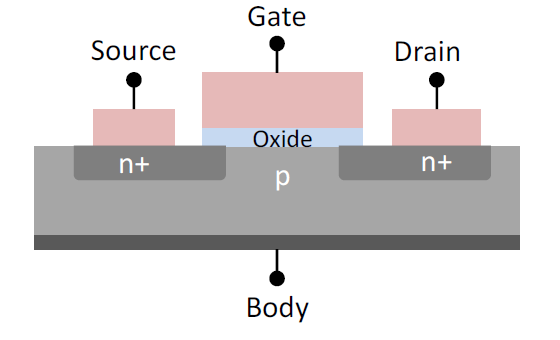
\includegraphics[width= 0.3\linewidth]{../figures/MOSFET.png}
		\label{fig:mosfet}
	\end{figure}
\end{frame}
% -----------------------------------------------
%---begin subsection----
\subsection{polymorphism of borophene}
\begin{frame}{polymorphism of borophene}
	\begin{figure}
		\centering
		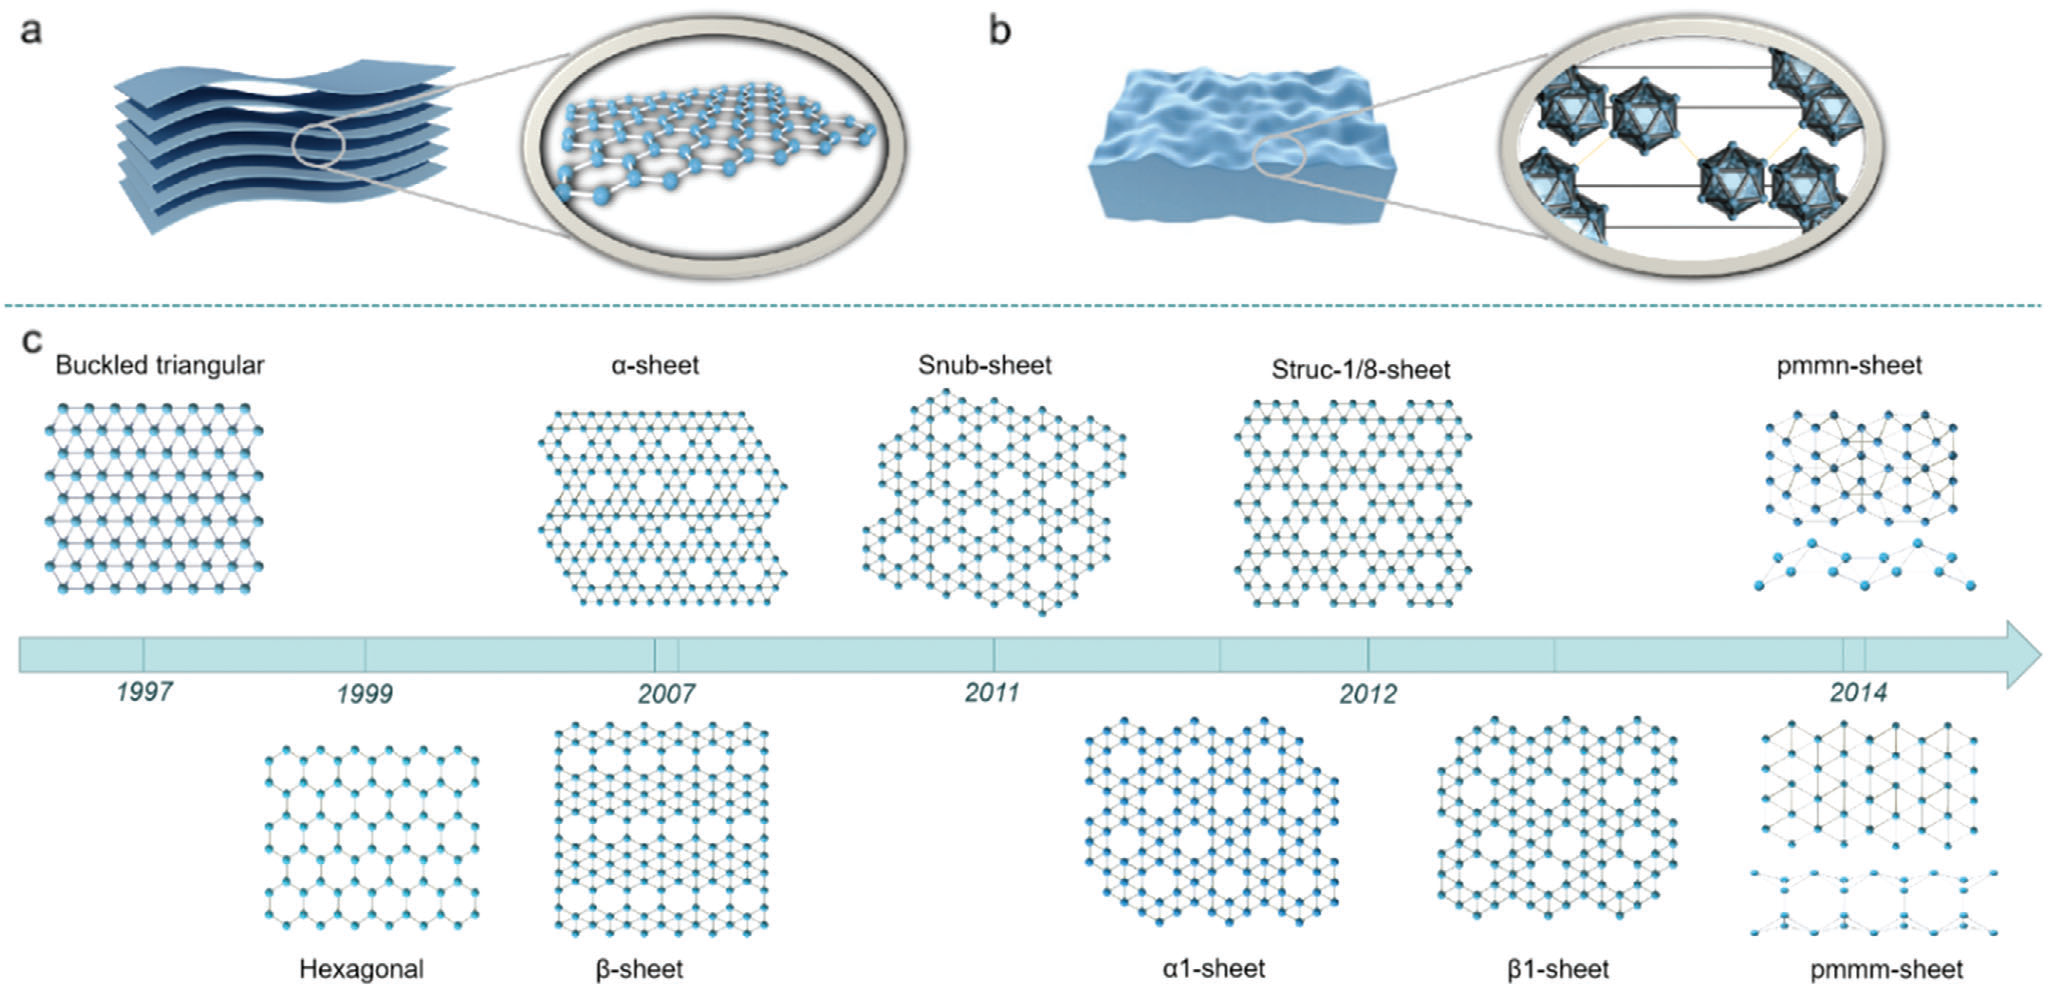
\includegraphics[width=\textwidth]{../figures/theory-borophene.png}
		\label{theoryborophene}
	\end{figure}
\end{frame}
% -----------------------------------------------
%end subsection
\subsection{Applications of borophene}
\begin{frame}{Applications of borophene}
	\begin{itemize}
		\item Biosensors for detecting glucose and other analytes.
		\item Contrast agents for high-resolution medical imaging
		\item Drug delivery systems with targeted material-cell interactions
		\item Implantable medical devices with improved safety and efficacy
		\item Cancer Therapy
		\item Hydrogen Storage
		\item Supercapacitors
		\item Batteries
	\end{itemize}
\end{frame}
% -----------------------------------------------
\begin{frame}{Applications of borophene}
	\begin{figure}[!h]
		\centering
		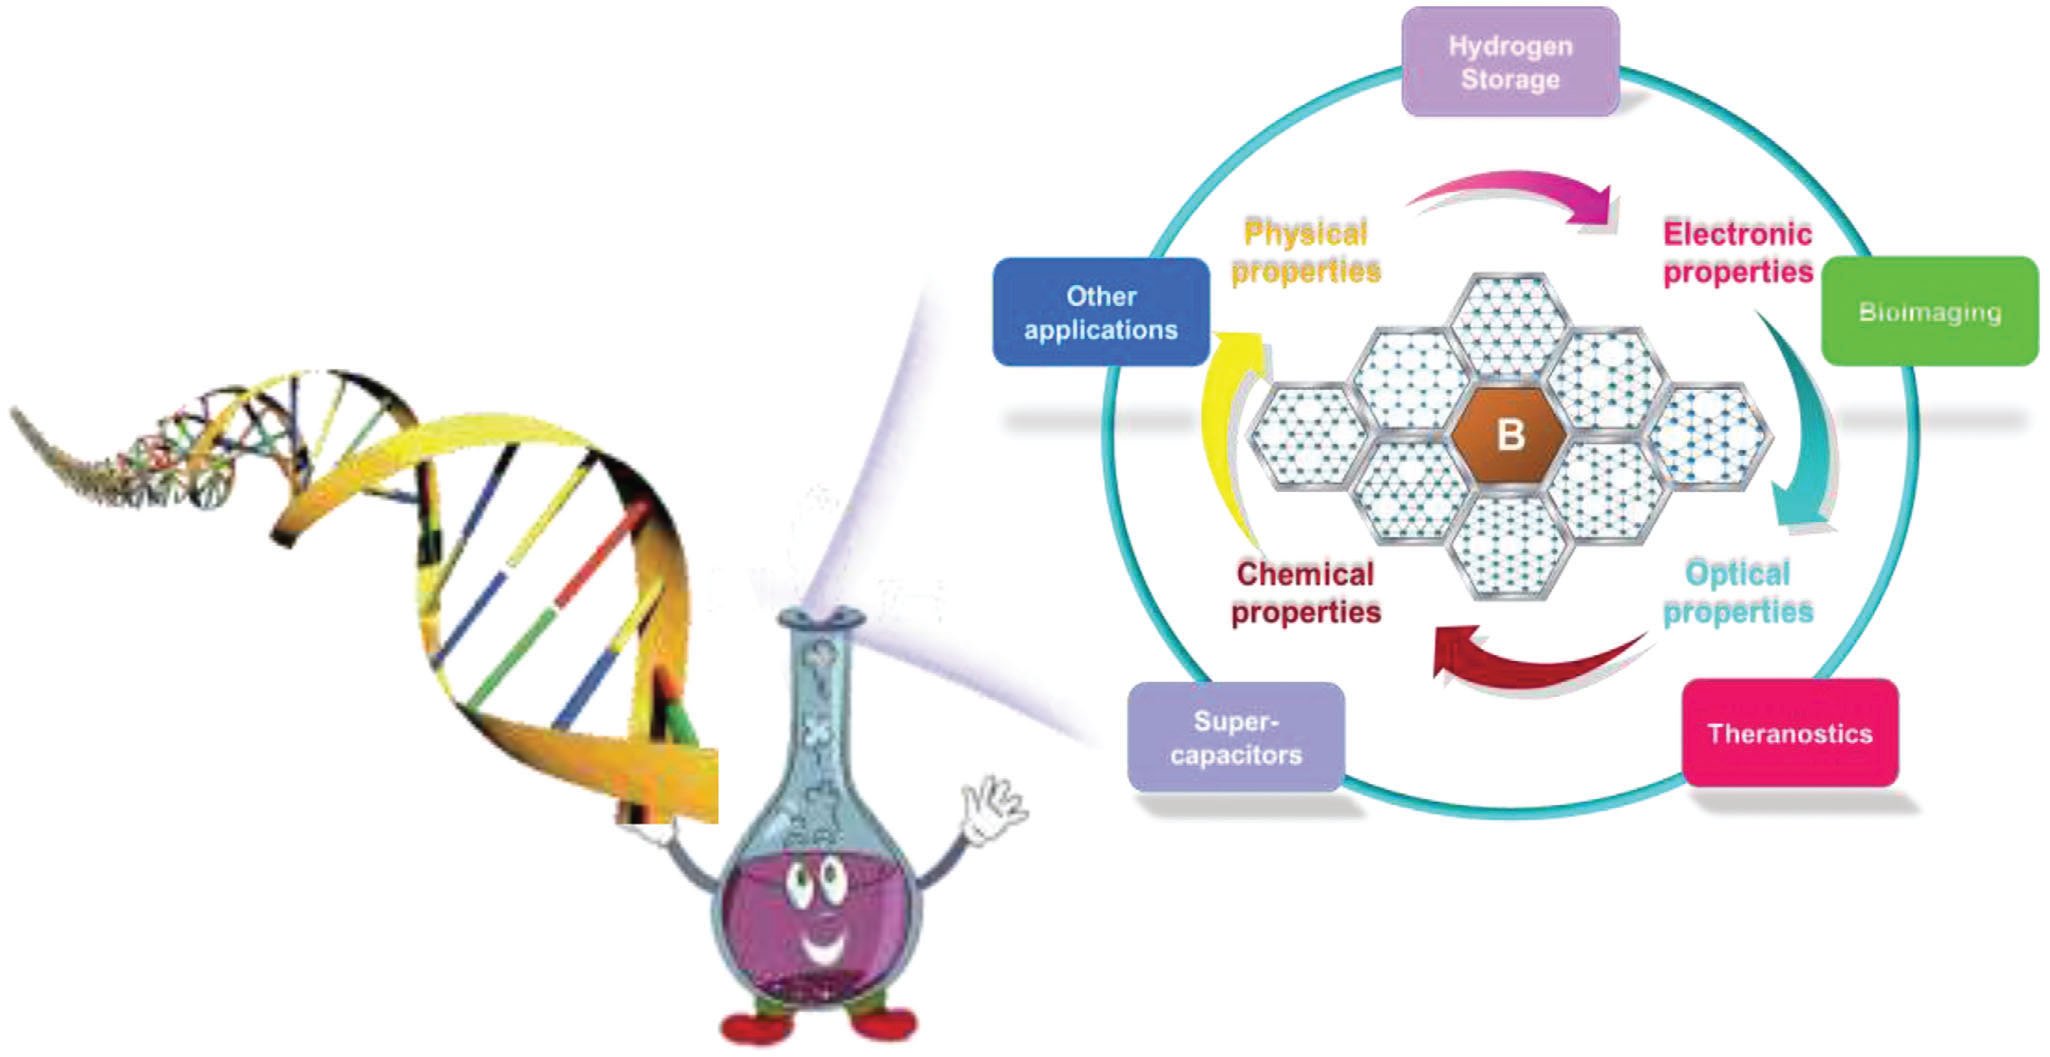
\includegraphics[width=\linewidth]{../figures/borophenedev.png}
		\label{fig:borophenedev}
	\end{figure}
\end{frame}
%end subsection
% -----------------------------------------------
\subsection{Topological Properties}
\begin{frame}{Topological Properties}
	\begin{columns}
		\begin{column}[t]{0.7\linewidth}
			\begin{itemize}
				\item Borophene has the potential to host topological Dirac cones similar to graphene, making it a promising light element for stable topological materials.
				\item Pmmn borophene is predicted to be the first 2D Dirac boron material with massless Dirac fermions and twisted Dirac cones.
				\item $\beta_{12}$ borophene, the first successfully synthesized non-honeycomb monolayer Dirac material, hosts Dirac fermions originating from its $p_z$ orbitals and can be split by periodic perturbations.
			\end{itemize}
		\end{column}
		\begin{column}[t]{0.5\linewidth}
			\begin{figure}
				\centering
				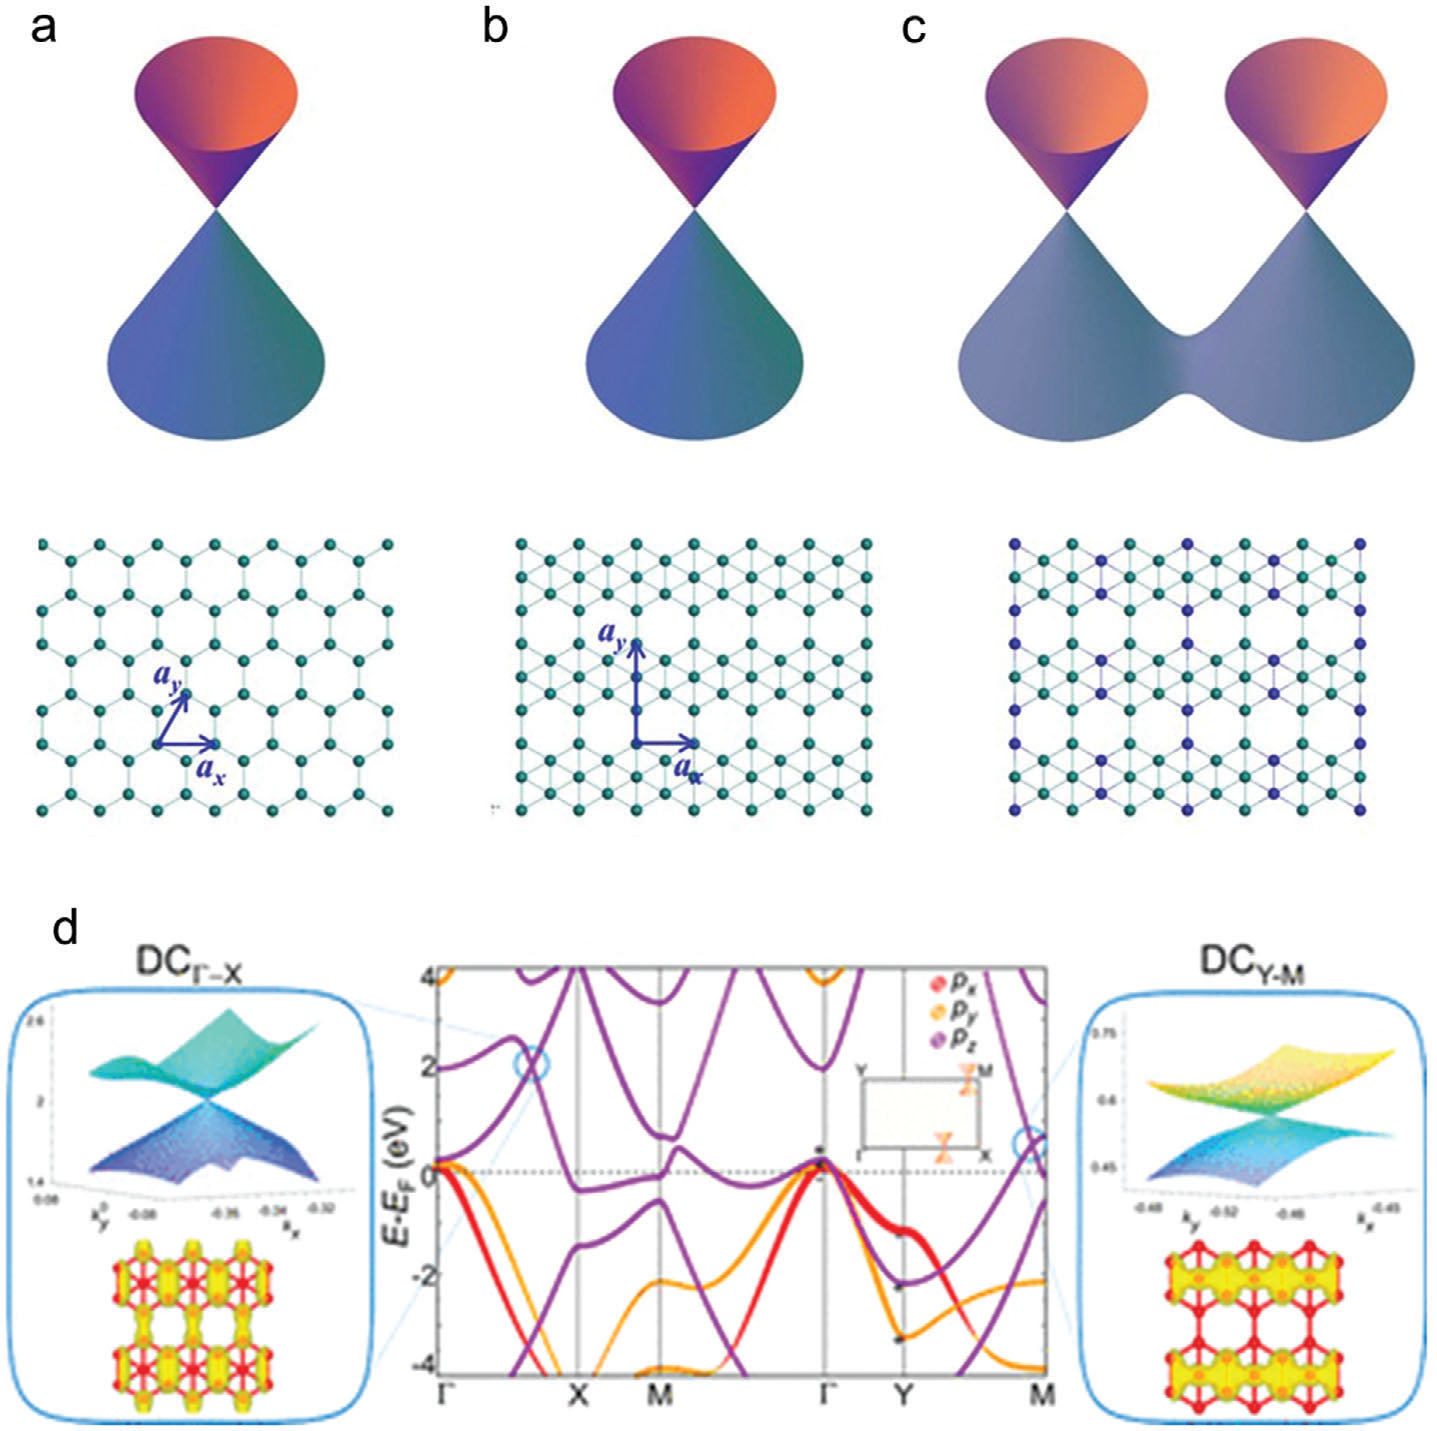
\includegraphics[width=\linewidth]{../figures/Diraccone.png}
			\end{figure}
		\end{column}
	\end{columns}
\end{frame}
%end subsection
% ----------------------------------------------
% \begin{frame}{Spin Current}
% 	\begin{figure}[!ht]
% 		\centering
% 		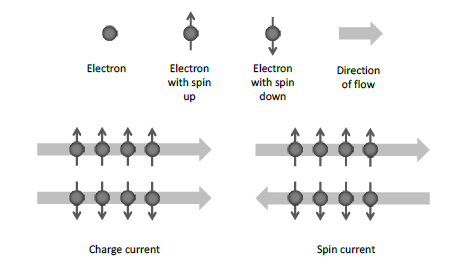
\includegraphics[width=0.7\linewidth]{../figures/spinchargecurent.png}
% 		\label{fig:spinchargecurent}
% 	\end{figure}
% \end{frame}
% ---------------------------------------
% \begin{frame}{MOSFET}
% 	\begin{figure}[!ht]
% 		\centering
% 		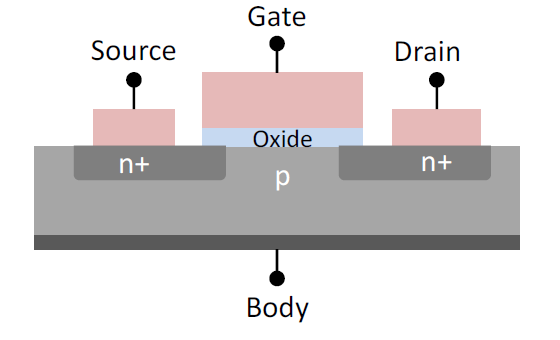
\includegraphics[width= 0.8\linewidth]{../figures/MOSFET.png}
% 		\label{fig:mosfet}
% 	\end{figure}
% \end{frame}
% ------------------------------------
% \begin{frame}{GrapheneFET}
% 	\begin{figure}[!ht]
% 		\centering
% 		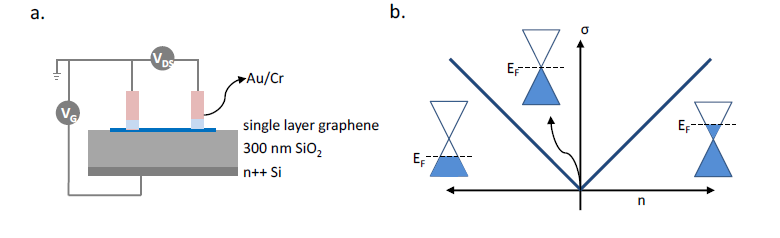
\includegraphics[width=\linewidth]{../figures/GrapheneFET.png}
% 		\label{fig:graphenefet}
% 	\end{figure}
% \end{frame}
% -----------------------------------------
% \begin{frame}{Spin Injections}
% 	\begin{figure}[!ht]
% 		\centering
% 		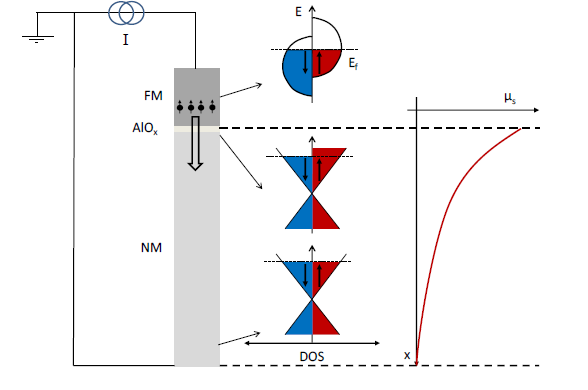
\includegraphics[width=\linewidth]{../figures/spininjection.png}
% 		\label{fig:spininjection}
% 	\end{figure}
% \end{frame}
% -----------------------------------------------
%-----end Introduction
%---begin section-------
% \section{Borophene}
% \begin{frame}{text here}
% 	text here
% \end{frame}
%---begin subsection----


%---begin subsection----
% \subsection{electrical properties}
% \begin{frame}{electricalproperties}
% 	\begin{figure}
% 		\centering
% 		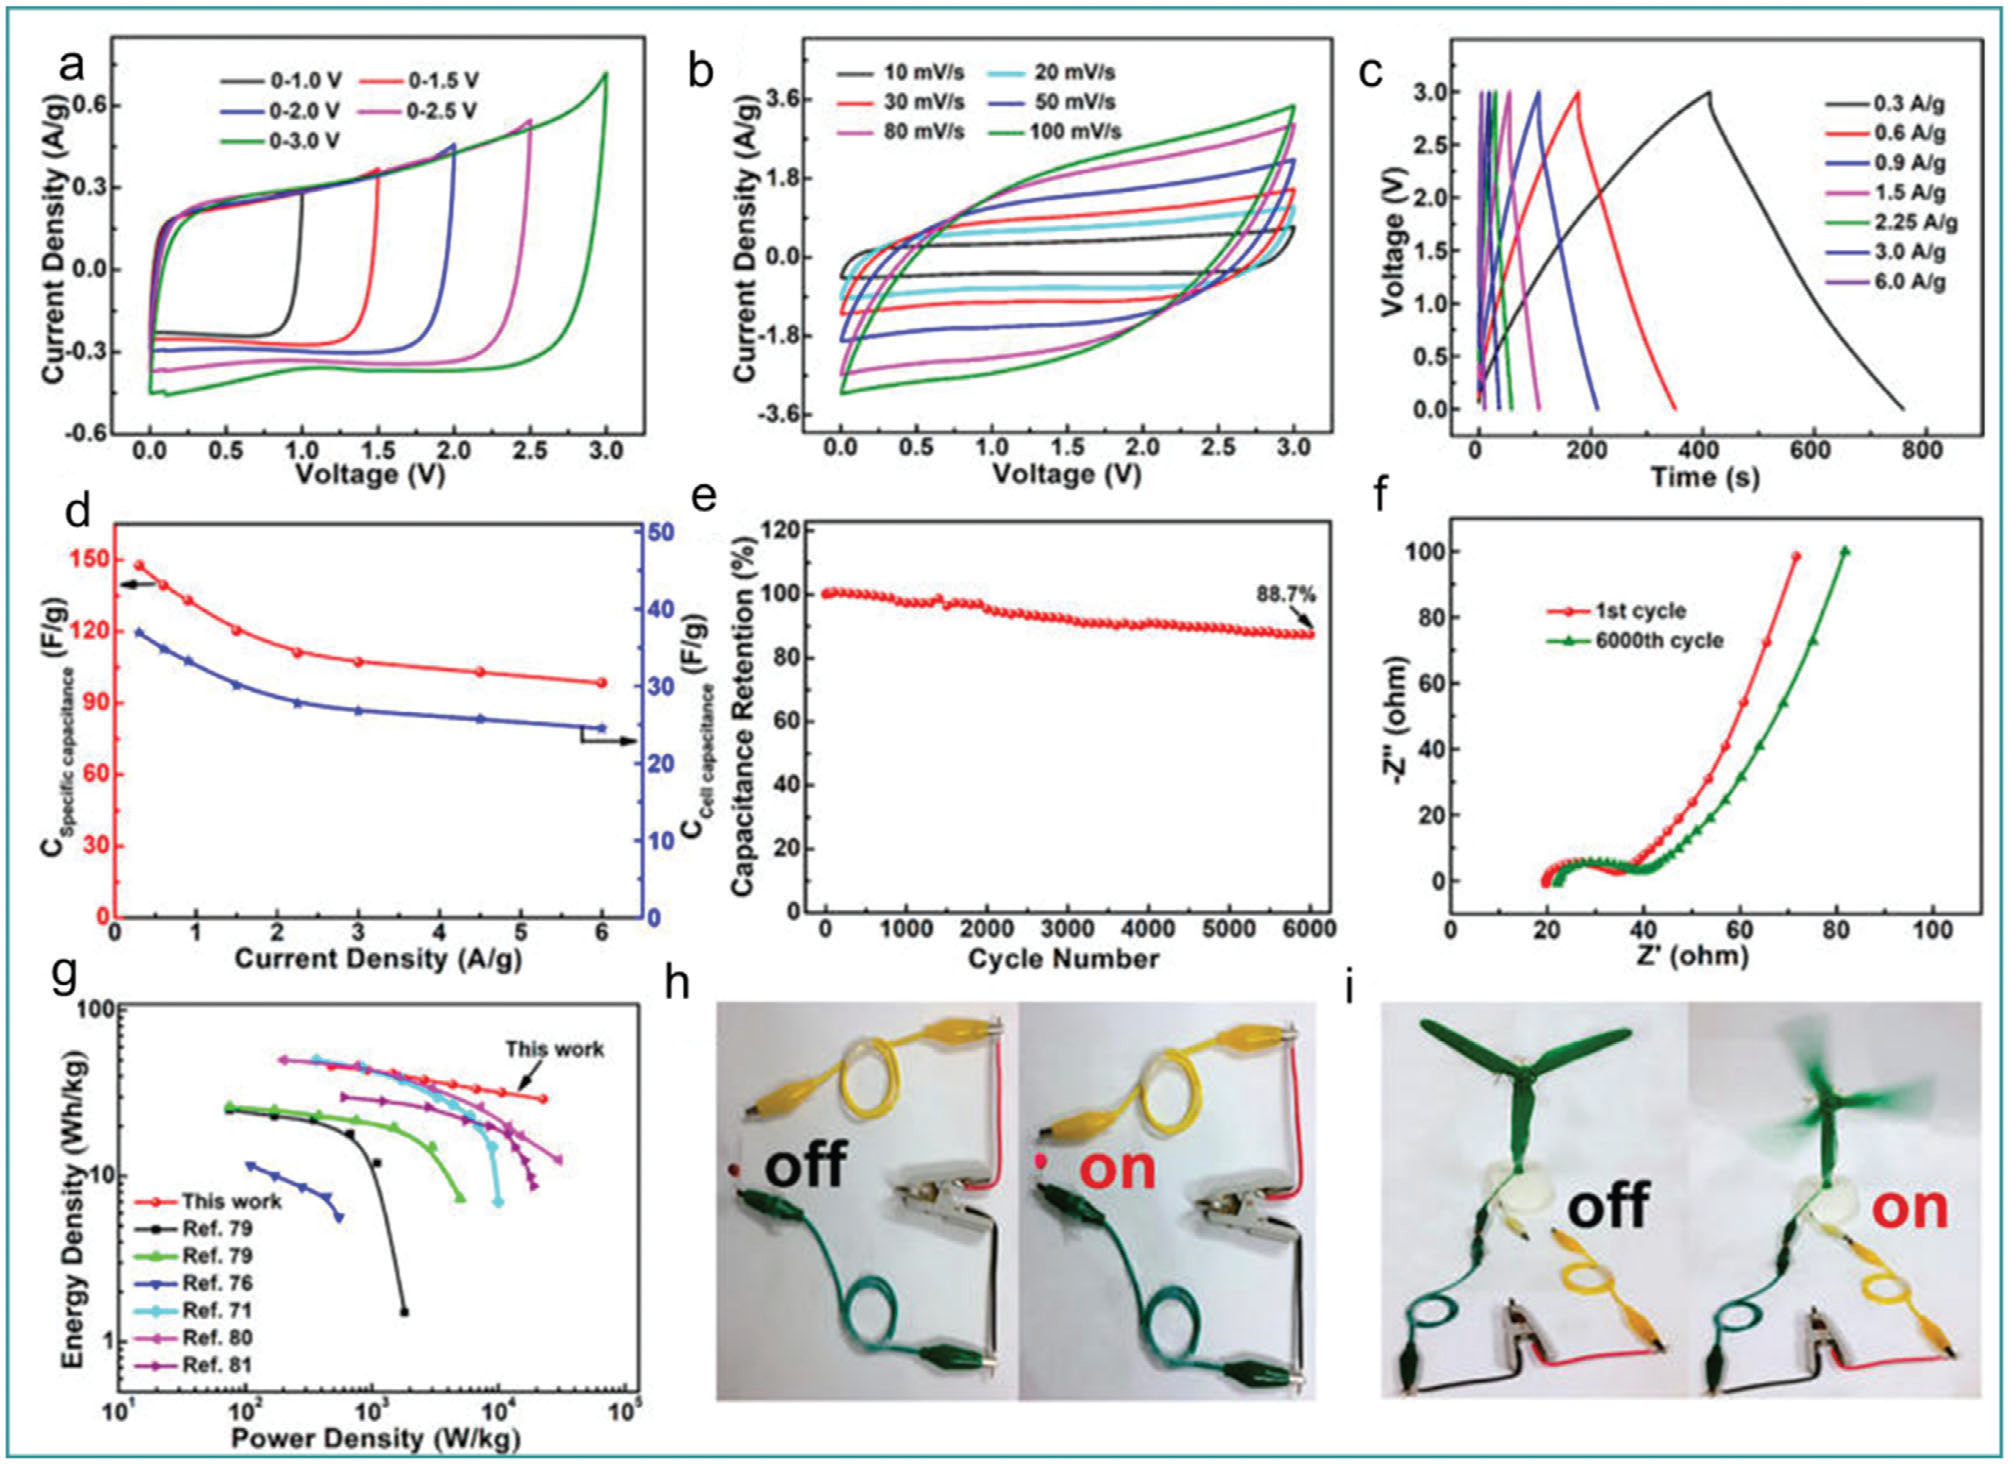
\includegraphics[width=0.5\linewidth]{../figures/electricalproperties.png}
% 		\label{fig:electricalproperties}
% 	\end{figure}
% \end{frame}
%end subsection
%---begin subsection----
% \subsection{absorbtion}
% \begin{frame}{absorbtion}
% 	\begin{figure}
% 		\centering
% 		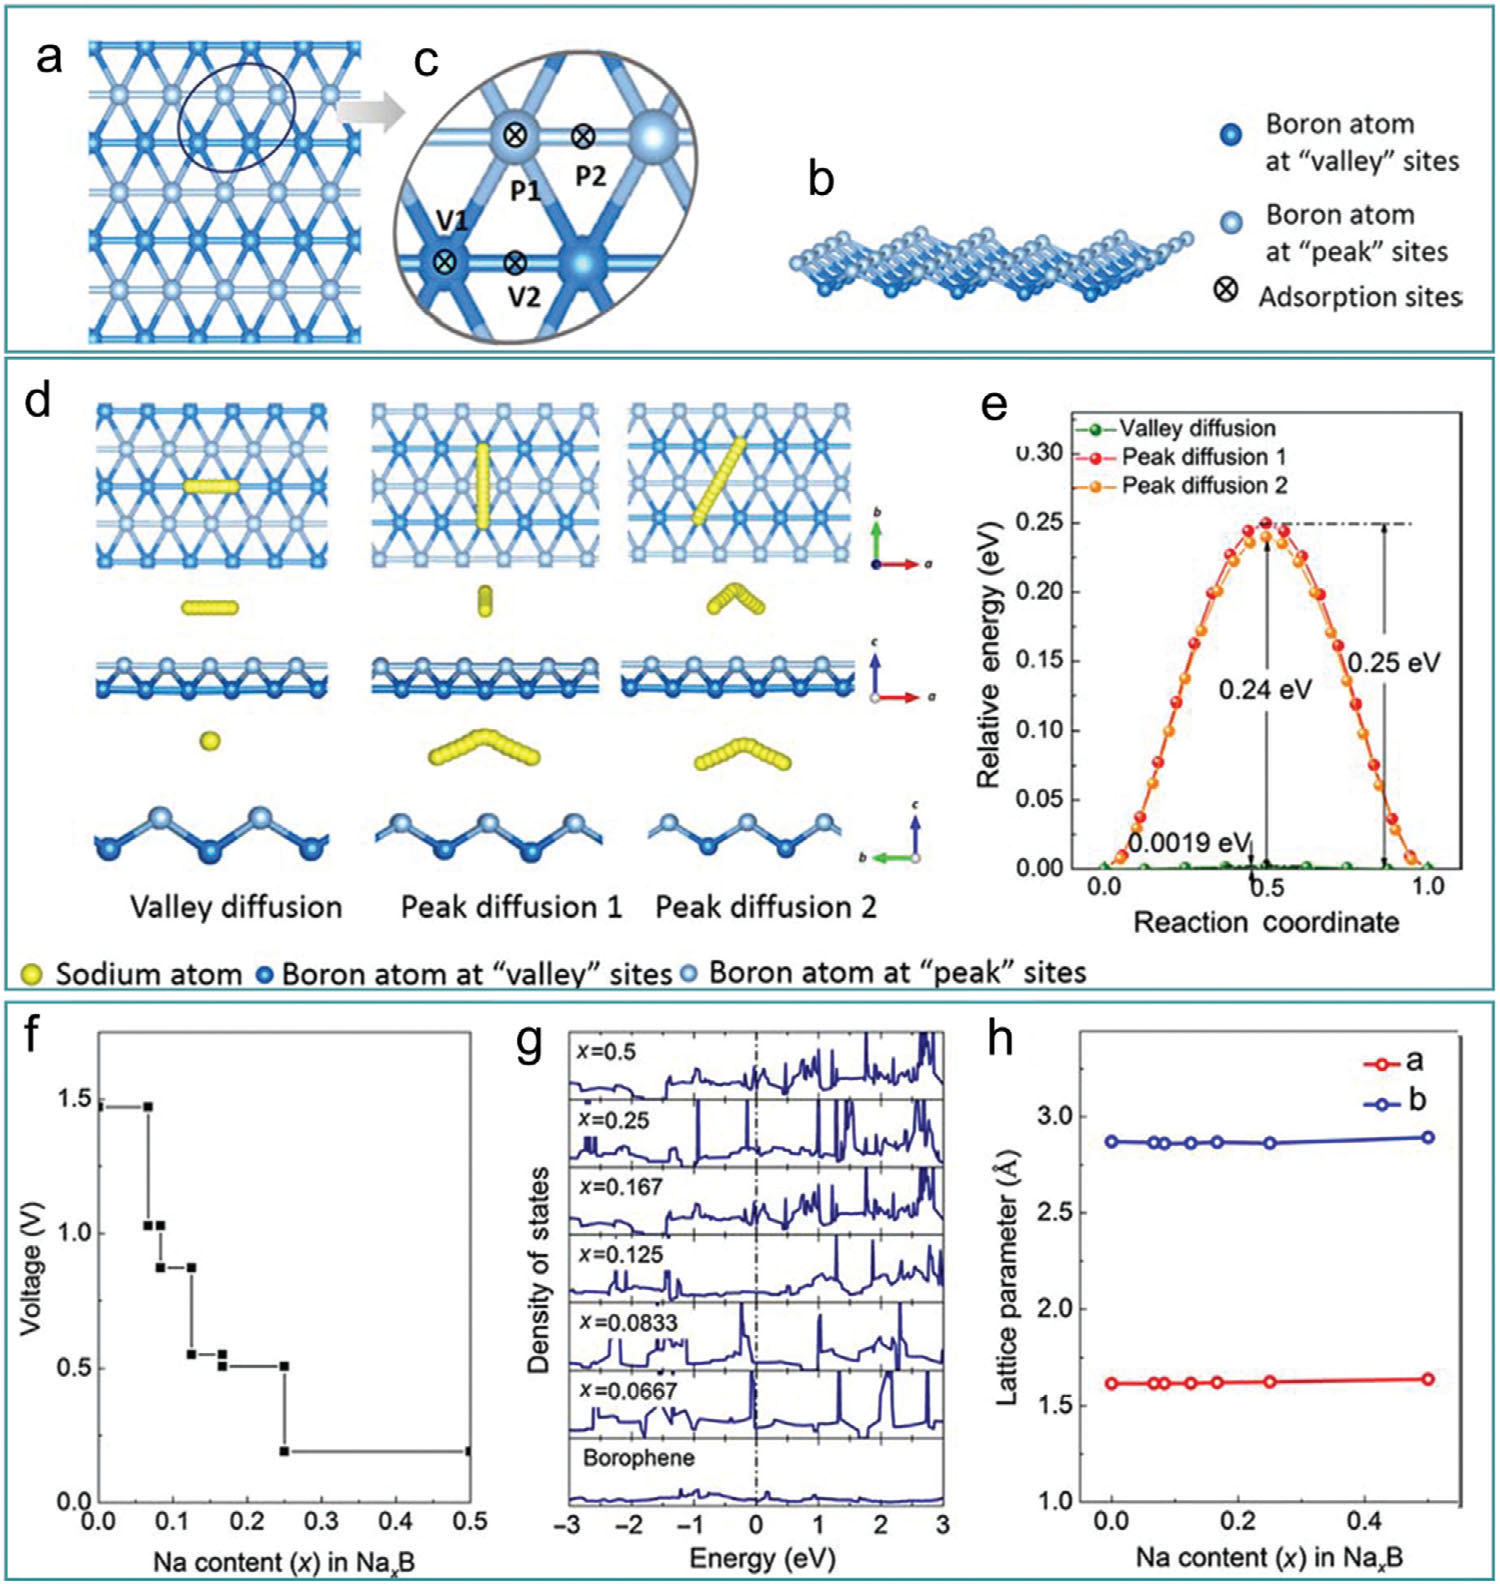
\includegraphics[width=0.5\linewidth]{../figures/absorbtion.png}
% 		\label{fig:absorbtion}
% 	\end{figure}
% \end{frame}
%end subsection
%---begin subsection----
% \subsection{alphasheet}
% \begin{frame}{alphasheet}
% 	\begin{figure}
% 		\centering
% 		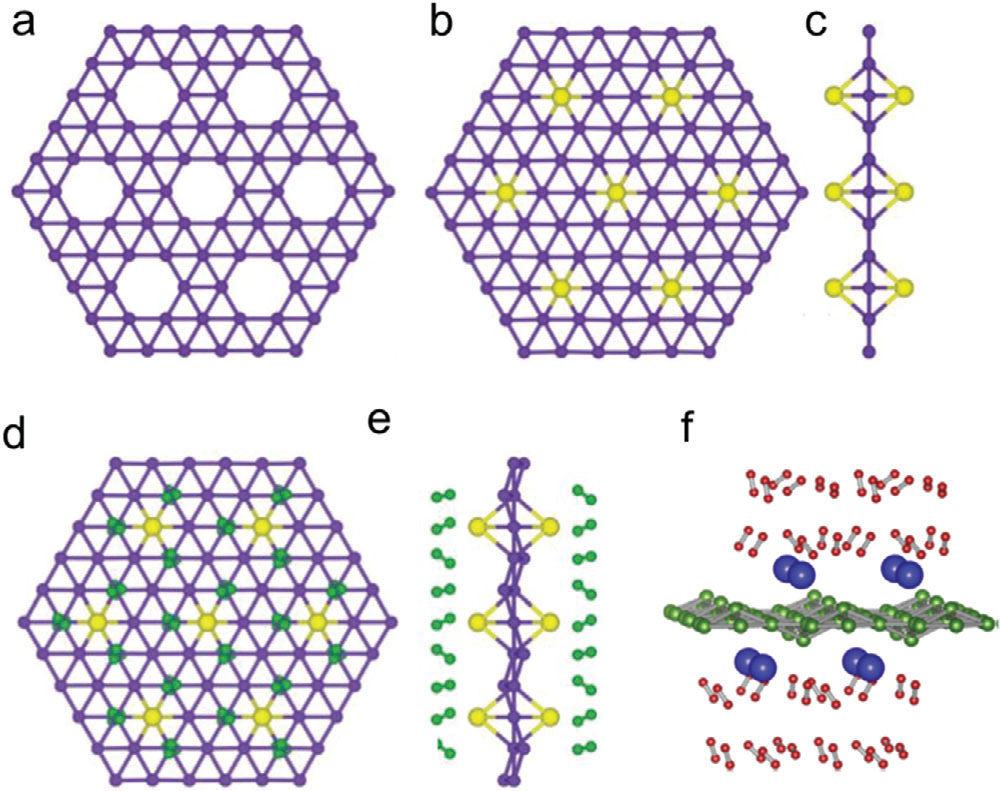
\includegraphics[width=0.5\linewidth]{../figures/alphasheet.png}
% 		\label{fig:alphasheet}
% 	\end{figure}
% \end{frame}
%end subsection
% \subsection{Multimodal}
% \begin{frame}{Multimodal}
% 	teest
% 	\begin{figure}
% 		\centering
% 		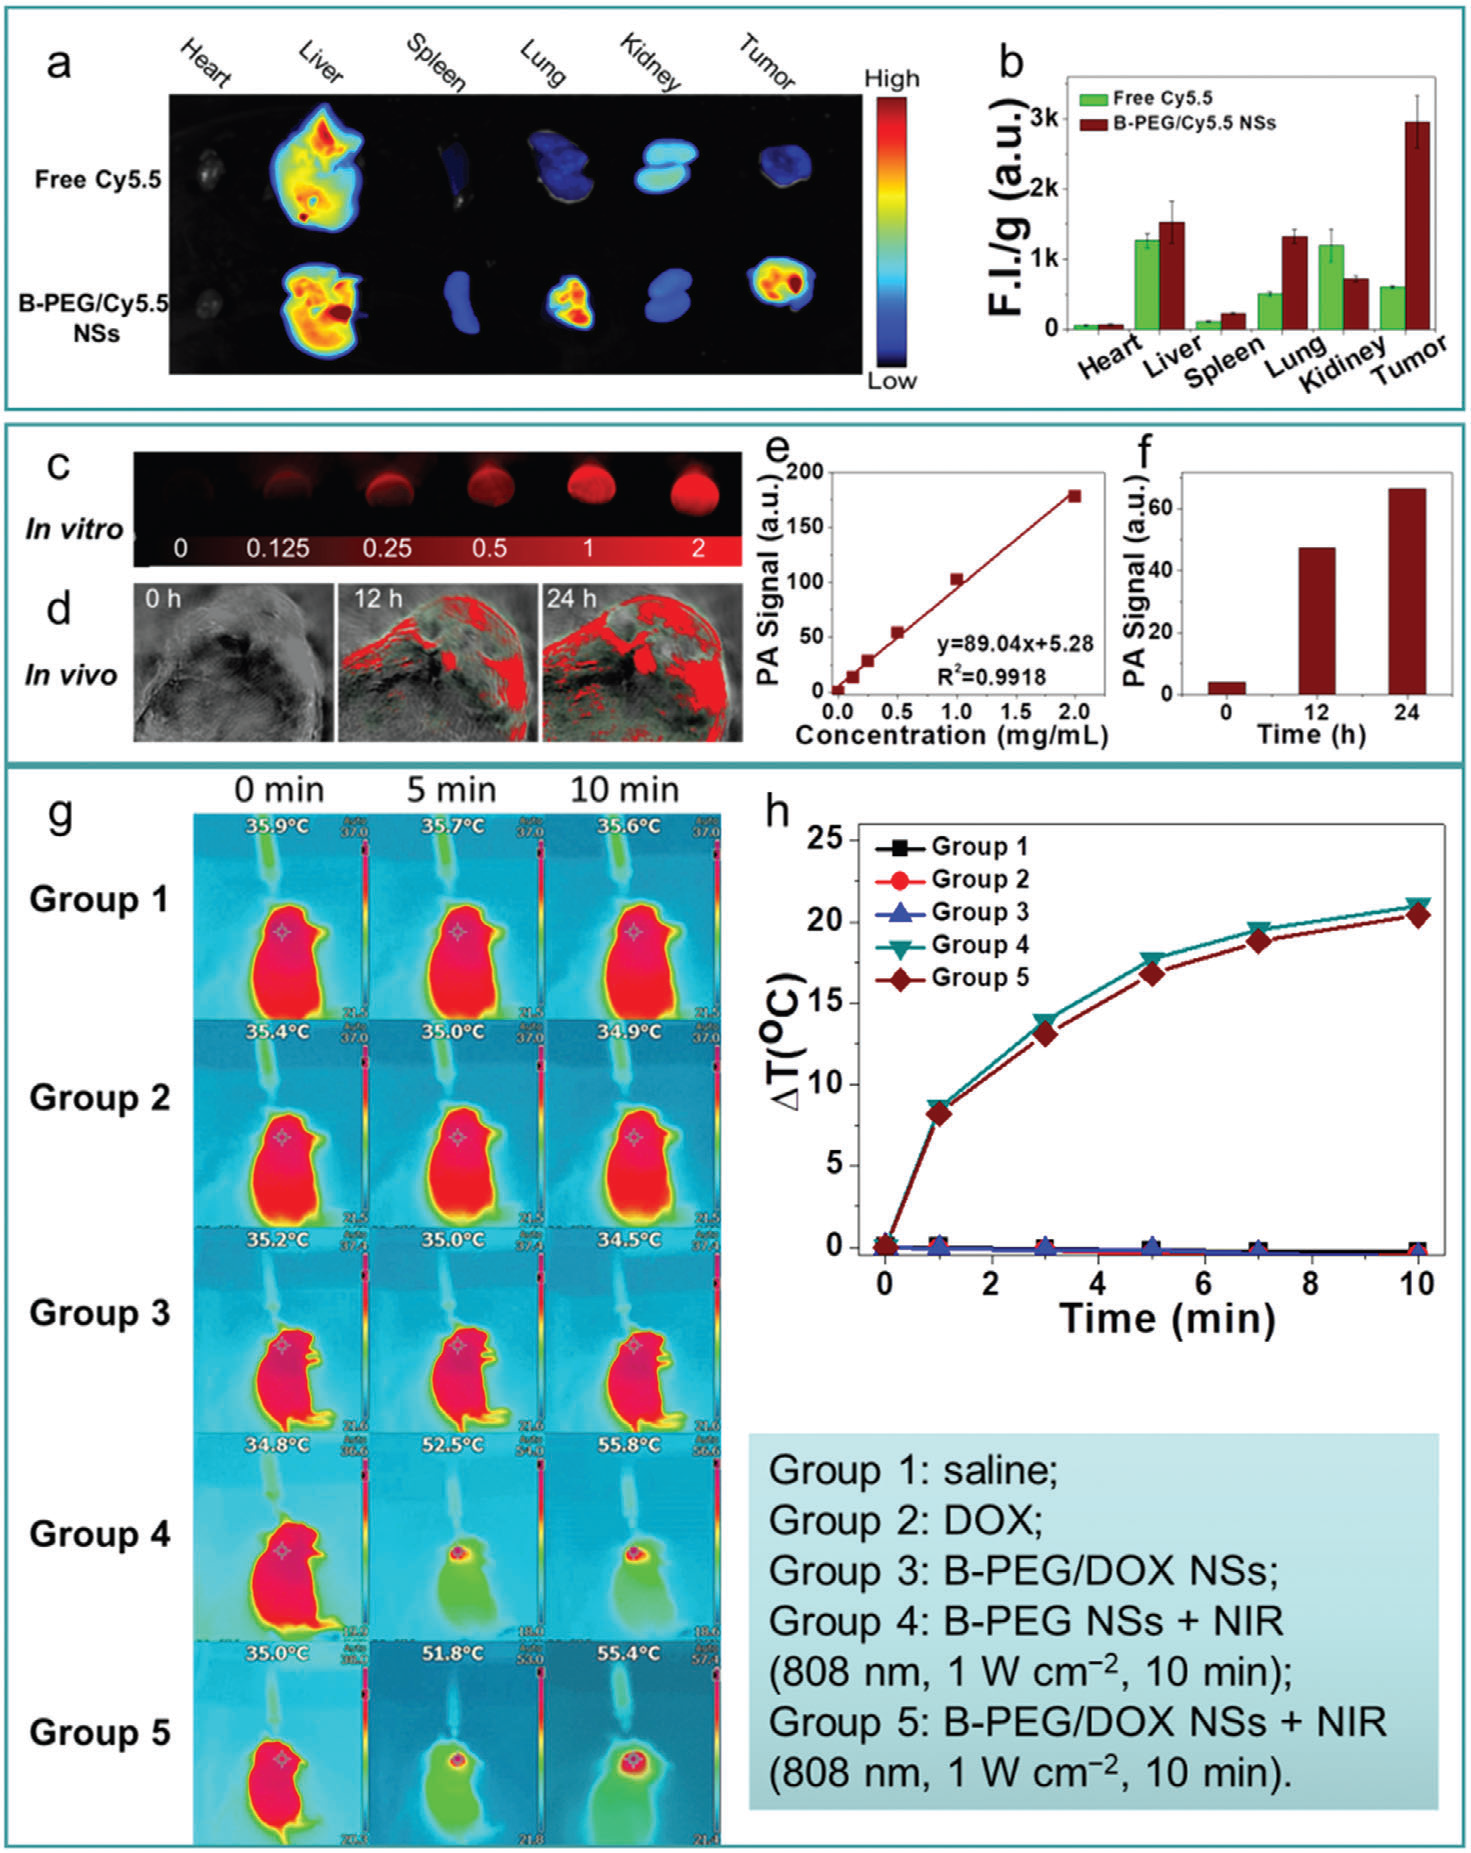
\includegraphics[width=0.5\linewidth]{../figures/Multimodal.png}
% 		\label{fig:Multimodal}
% 	\end{figure}
% \end{frame}
%end subsection
% \subsection{UV}
% \begin{frame}{UV}
% 	teest
% 	\begin{figure}
% 		\centering
% 		\includegraphics[width=0.5\linewidth]{../figures/UV.png}
% 		\label{fig:UV}
% 	\end{figure}
% \end{frame}
%end subsection
%end subsection

%---end section----
%---begin section-------
\section{Methodes}
\begin{frame}{NEGF Method}
	\begin{columns}
		\begin{column}[t]{0.5\linewidth}
			\begin{itemize}
				\item Established in the 1960s through the work of Schwinger, Kadanoff, Baym, Keldysh and others.
				\item These equations have been used to discuss many problems of great interest, such as:\begin{itemize}
					\item Quantized conductance
					\item (Integer) quantum Hall effect
					\item Anderson localization
					\item Resonant tunneling
					\item Spin transport
				\end{itemize}
			\end{itemize}
		\end{column}
		\begin{column}[t]{0.5\linewidth}
			\begin{figure}
				\centering
				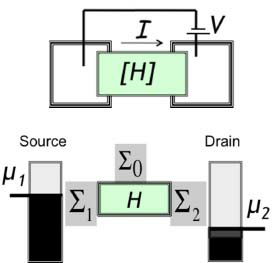
\includegraphics[width=\linewidth]{../figures/NEGF-model.png}
				\label{fig:NEGF-model}
			\end{figure}
		\end{column}
	\end{columns}
\end{frame}
% -----------------------------------------------
\begin{frame}{Green Function}
	\begin{figure}
		\centering
		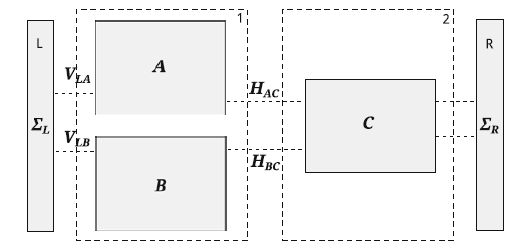
\includegraphics[width=0.7\linewidth]{../figures/multiconnectedgreen.png}
		\label{fig:multiconnectedgreen}
	\end{figure}
	\begin{equation}
		\begin{aligned}
			  & \left( \begin{matrix}
			   {{G}_{A}} & {{G}_{AB}} & {{G}_{AC}}  \\
			   {{G}_{BA}} & {{G}_{B}} & {{G}_{BC}}  \\
			   {{G}_{LA}} & {{G}_{LB}} & {{G}_{L}}  \\
			\end{matrix} \right)=\left( \begin{matrix}
			   G_{A}^{0} & 0 & 0  \\
			   0 & G_{B}^{0} & 0  \\
			   0 & 0 & G_{L}^{0}  \\
			\end{matrix} \right)+ \\ 
			 & \left( \begin{matrix}
			   G_{A}^{0} & 0 & 0  \\
			   0 & G_{B}^{0} & 0  \\
			   0 & 0 & G_{L}^{0}  \\
			\end{matrix} \right)\left( \begin{matrix}
			   0 & 0 & {{V}_{AL}}  \\
			   0 & 0 & {{V}_{BL}}  \\
			   {{V}_{LA}} & {{V}_{LB}} & 0  \\
			\end{matrix} \right)\left( \begin{matrix}
			   {{G}_{A}} & {{G}_{AB}} & {{G}_{AC}}  \\
			   {{G}_{BA}} & {{G}_{B}} & {{G}_{BC}}  \\
			   {{G}_{LA}} & {{G}_{LB}} & {{G}_{L}}  \\
			\end{matrix} \right). \\ 
		\end{aligned}
		\label{eq:expandmultigrren}
	\end{equation}
\end{frame}
% ----------------------------------------------
%---end section----
\begin{frame}{NEGF}
	\begin{figure}
    \centering
    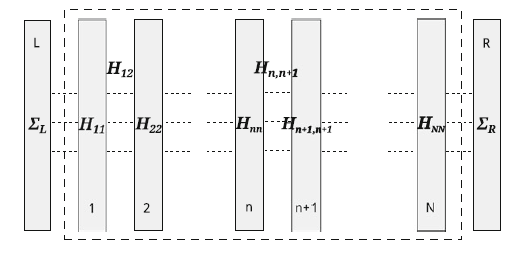
\includegraphics[width=0.45\linewidth]{../figures/iteration.png}
    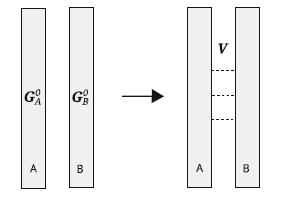
\includegraphics[width=0.45\linewidth]{../figures/greendyson.png}\\
    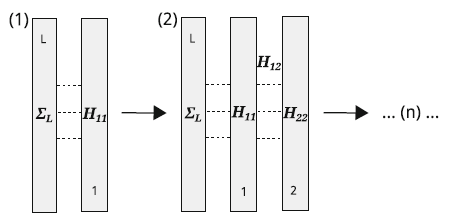
\includegraphics[width=0.45\linewidth]{../figures/iterationchannelgreen.png}
    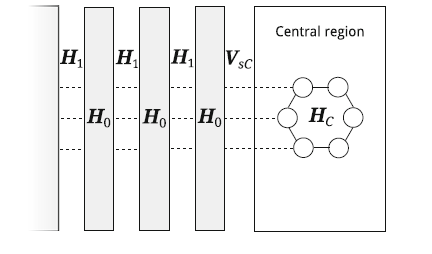
\includegraphics[width=0.45\linewidth]{../figures/leaditerationgreen.png}
    \label{fig:greendyson}
\end{figure}
\end{frame}
% -----------------------------------------------
\begin{frame}{Green Function}
	\begin{equation}
		\left( \begin{matrix}
			   {{G}_{A}} & {{G}_{AB}}  \\
			   {{G}_{BA}} & {{G}_{B}}  \\
			\end{matrix} \right)=\left( \begin{matrix}
			   G_{A}^{0} & 0  \\
			   0 & G_{B}^{0}  \\
			\end{matrix} \right)+\left( \begin{matrix}
			   G_{A}^{0} & 0  \\
			   0 & G_{B}^{0}  \\
			\end{matrix} \right)\left( \begin{matrix}
			   0 & {{V}_{AB}}  \\
			   {{V}_{AB}} & 0  \\
			\end{matrix} \right)\left( \begin{matrix}
			   {{G}_{A}} & {{G}_{AB}}  \\
			   {{G}_{BA}} & {{G}_{B}}  \\
			\end{matrix} \right),
	\end{equation}
	\begin{equation}
		\begin{split}
			  & {{G}_{A}}=G_{A}^{0}+G_{A}^{0}{{V}_{AB}}{{G}_{BA}}\qquad {{G}_{AB}}=G_{A}^{0}{{V}_{AB}}{{G}_{B}} \\ 
			 & {{G}_{BA}}=G_{B}^{0}{{V}_{BA}}{{G}_{A}}\qquad \qquad {{G}_{B}}=G_{B}^{0}+G_{B}^{0}{{V}_{BA}}{{G}_{AB}} \\ 
			 & {{G}_{A}}=G_{A}^{0}+G_{A}^{0}{{V}_{AB}}{{G}_{BA}}\qquad {{G}_{AB}}=G_{A}^{0}{{V}_{AB}}{{G}_{B}} \\ 
			& {{G}_{BA}}=G_{B}^{0}{{V}_{BA}}{{G}_{A}}\qquad \qquad {{G}_{B}}=G_{B}^{0}+G_{B}^{0}{{V}_{BA}}{{G}_{AB}} \\ 
		\end{split}
		\label{eq:greenselfenergy}
	\end{equation}
	\begin{equation}
		\left( \begin{matrix}
			   {{\Sigma }_{AA}} & {{\Sigma }_{AB}}  \\
			   {{\Sigma }_{BA}} & {{\Sigma }_{BB}}  \\
			\end{matrix} \right)=\left( \begin{matrix}
			   {{V}_{AL}}G_{L}^{0}{{V}_{LA}} & {{V}_{AL}}G_{L}^{0}{{V}_{LB}}  \\
			   {{V}_{BL}}G_{L}^{0}{{V}_{LA}} & {{V}_{BL}}G_{L}^{0}{{V}_{LB}}  \\
			\end{matrix} 
		\right).
	\end{equation}
	\begin{equation}
		{{G}_{C}}={{\left[ E-{{H}_{C}}-{{\Sigma }_{R}}-{{H}_{CA}}G_{A}^{\to (1)}\ {{H}_{AC}}-{{H}_{CB}}G_{B}^{\to (1)}\ {{H}_{BC}} \right]}^{-1}}.
	\end{equation}
\end{frame}
% ----------------------------------------------
\begin{frame}{recursive iteration method}
	\begin{equation}
		\begin{aligned}
			&{{A}^{(0)}}={{H}_{1}},\\
			&{{B}^{(0)}}=H_{1}^{\dagger},\\
			&{{C}^{(0)}}=E-{{H}_{0}},\\
			&{{D}^{(0)}}=E-{{H}_{0}},
		\end{aligned}
	\end{equation}
	\begin{equation}
		\begin{aligned}
			&{{A}^{(n)}}={{A}^{(n-1)}}{{({{D}^{(n-1)}})}^{-1}}{{A}^{(n-1)}},\\
			&{{B}^{(n)}}={{B}^{(n-1)}}{{({{D}^{(n-1)}})}^{-1}}{{B}^{(n-1)}},\\
			&{{C}^{(n)}}={{C}^{(n-1)}}-{{A}^{(n-1)}}{{({{D}^{(n-1)}})}^{-1}}{{B}^{(n-1)}},\\
			&{{D}^{(n)}}={{D}^{(n-1)}}-{{A}^{(n-1)}}{{({{D}^{(n-1)}})}^{-1}}{{B}^{(n-1)}}-{{B}^{(n-1)}}{{({{D}^{(n-1)}})}^{-1}}{{A}^{(n-1)}},
		\end{aligned}
	\end{equation}
\end{frame}
%---end section----
% --------------------------------------------
% \begin{frame}{text here}
% 	\begin{equation}
% 		\left( \begin{matrix}
% 			   {{\Sigma }_{AA}} & {{\Sigma }_{AB}}  \\
% 			   {{\Sigma }_{BA}} & {{\Sigma }_{BB}}  \\
% 			\end{matrix} \right)=\left( \begin{matrix}
% 			   {{V}_{AL}}G_{L}^{0}{{V}_{LA}} & {{V}_{AL}}G_{L}^{0}{{V}_{LB}}  \\
% 			   {{V}_{BL}}G_{L}^{0}{{V}_{LA}} & {{V}_{BL}}G_{L}^{0}{{V}_{LB}}  \\
% 			\end{matrix} 
% 		\right).
% 	\end{equation}
% 	\begin{equation}
% 		{{G}_{C}}={{\left[ E-{{H}_{C}}-{{\Sigma }_{R}}-{{H}_{CA}}G_{A}^{\to (1)}\ {{H}_{AC}}-{{H}_{CB}}G_{B}^{\to (1)}\ {{H}_{BC}} \right]}^{-1}}.
% 	\end{equation}
% \end{frame}
% \begin{frame}{text here}
% 	\begin{equation}
% 		\begin{aligned}
% 			&{{A}^{(0)}}={{H}_{1}},\\
% 			&{{B}^{(0)}}=H_{1}^{\dagger},\\
% 			&{{C}^{(0)}}=E-{{H}_{0}},\\
% 			&{{D}^{(0)}}=E-{{H}_{0}},
% 		\end{aligned}
% 	\end{equation}
% 	\begin{equation}
% 		\begin{aligned}
% 			&{{A}^{(n)}}={{A}^{(n-1)}}{{({{D}^{(n-1)}})}^{-1}}{{A}^{(n-1)}},\\
% 			&{{B}^{(n)}}={{B}^{(n-1)}}{{({{D}^{(n-1)}})}^{-1}}{{B}^{(n-1)}},\\
% 			&{{C}^{(n)}}={{C}^{(n-1)}}-{{A}^{(n-1)}}{{({{D}^{(n-1)}})}^{-1}}{{B}^{(n-1)}},\\
% 			&{{D}^{(n)}}={{D}^{(n-1)}}-{{A}^{(n-1)}}{{({{D}^{(n-1)}})}^{-1}}{{B}^{(n-1)}}-{{B}^{(n-1)}}{{({{D}^{(n-1)}})}^{-1}}{{A}^{(n-1)}},
% 		\end{aligned}
% 	\end{equation}
% \end{frame}
%---end section----
\section{Charge Conductance}
% ----------------------------------------------
% \begin{frame}
% 	\begin{columns}
% 		\begin{column}[t]{0.5\linewidth}
			
% 		\end{column}
% 		\begin{column}[t]{0.5\linewidth}
% 			\begin{table}
% 				\centering
% 				\caption{The $\beta_{12}$-borophene hoping parameters introduced by Ezawa\cite{Ezawa2017Triplet}\label{jlab1}}
% 				\resizebox{\textwidth}{!}{\begin{tabular}{cccccccc}
% 				\toprule
% 				 & H & INS & IS &
% 				 & H & INS & IS\\
% 				\midrule
% 				$\varepsilon_a$& 0 &  0.196 &  0.196 & $t_{ab}=t_{de}$& -2 & -2.04 & -2.04 \\
% 				$\varepsilon_b$& 0 & -0.058 & -0.058 & $t_{ac}=t_{ce}$& -2 & -1.79 & -1.79 \\
% 				$\varepsilon_c$& 0 & -0.845 & -0.845 & $t_{ae}$& -2 & -2.12 & -2.12   \\
% 				$\varepsilon_d$& 0 &  0.196 & -0.058 & $t_{bc}=t_{cd}$& -2 & -1.84 & -1.84 \\
% 				$\varepsilon_e$& 0 & -0.058 &  0.196 & $t_{bd}$& -2 & -1.91 & -1.91  \\
% 				\bottomrule
% 				\end{tabular}}
% 				\end{table}
% 		\end{column}
% 	\end{columns}
% \end{frame}
% %---begin subsection--------------------------------------
\subsection{Outline of charge conductance}
% -----------------------------------------------
\begin{frame}{Conductance of $\beta_{12}$ Borophene Nanoribbons}
	\begin{itemize}
		\item Conductance of borophene $\beta_{12}$ nanoribbons (BNRs) studied using non-equilibrium Green's function (NEGF) method and tight-binding Hamiltonian
		\item Conductance depends on:
		\begin{itemize}
			\item Width of the ribbons
			\item Type of ribbon edges
		\end{itemize}
		\item Hidden honeycomb lattice within $\beta_{12}$ borophene.
		\item Single defects
		\item Anderson localization
	\end{itemize}
	\begin{figure}[!ht]
		\centering
		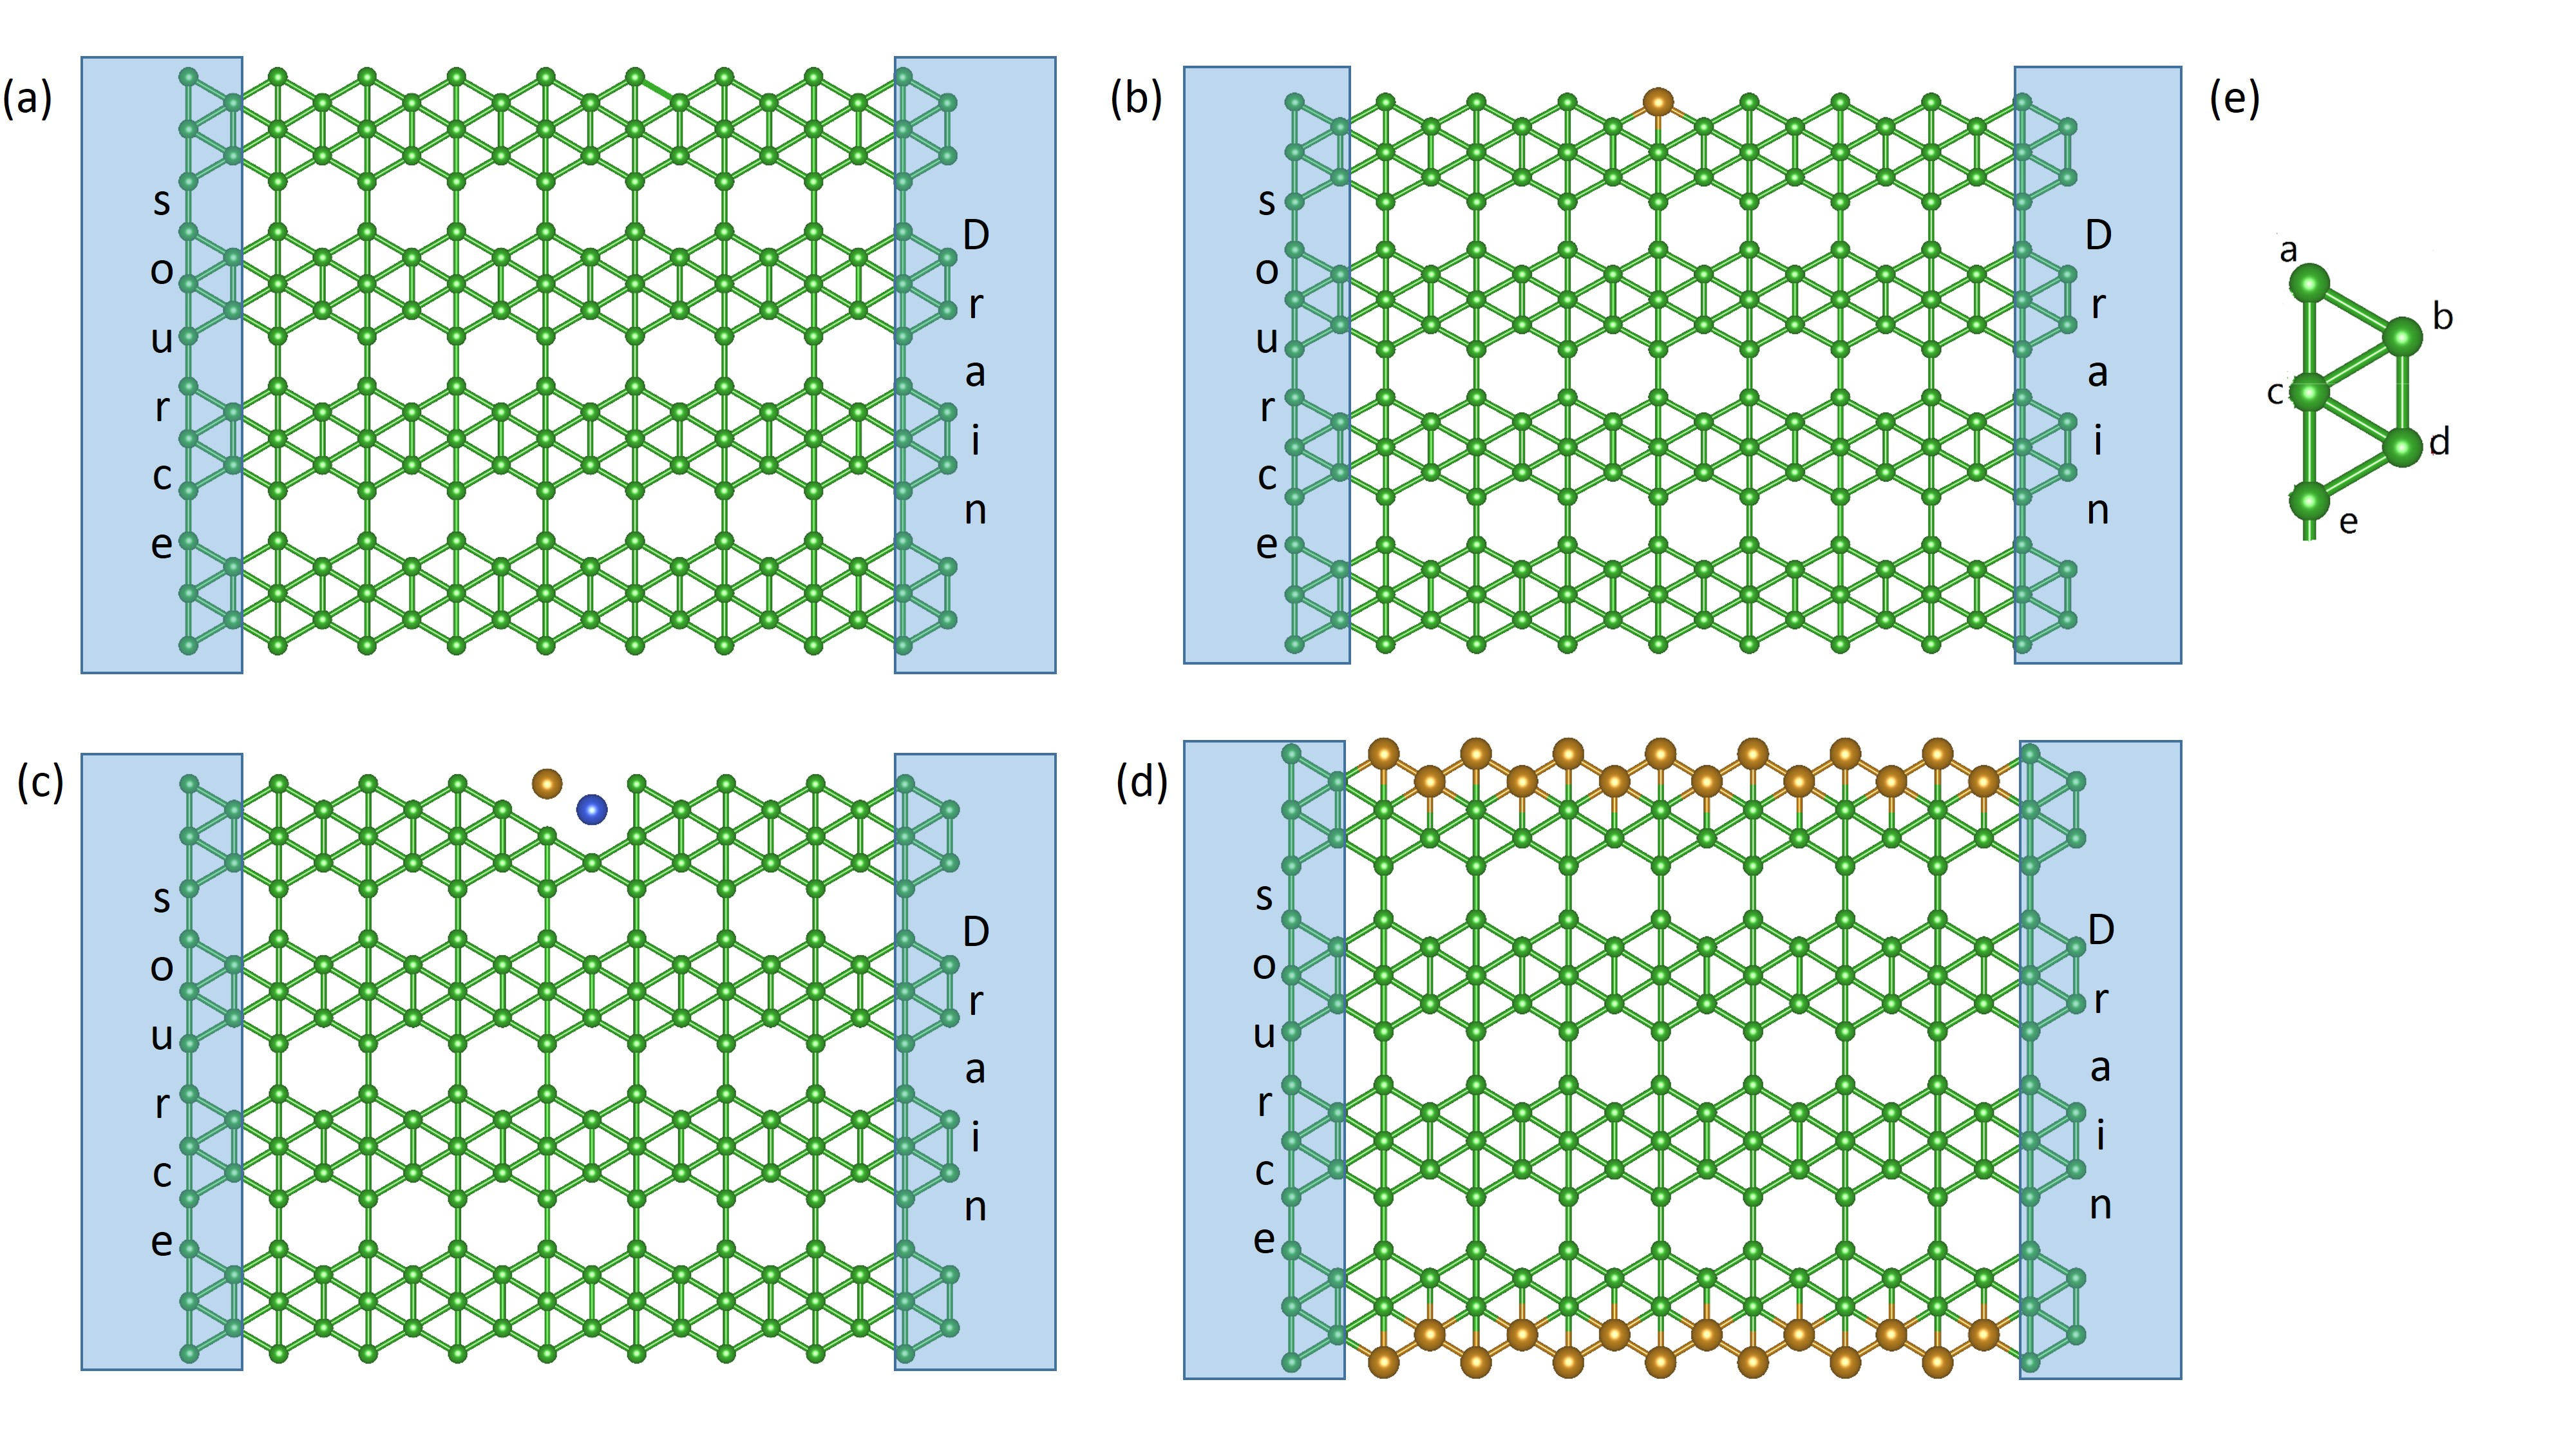
\includegraphics[width=.5\linewidth]{../figures/borophene_structure(3).JPG}
		\label{fig:borophene}
	  \end{figure}
\end{frame}
% end of subsection
% -----------------------------------------------
\subsection{Conductance VS Width}
% -----------------------------------------------
\begin{frame}{Transmission Spectra of Pristine Borophene Nanoribbons}
	\begin{itemize}
		\item Transmission spectra of pristine borophene nanoribbons (BNRs) show a well-known stepwise structure
		\item Height of the steps corresponds to the number of energy bands passing through a given energy
		\item Unlike graphene nanoribbons (GNRs), the number of conductance channels at the Fermi energy in BNRs does not remain constant
		\item Number of conductance channels at the Fermi energy increases with increasing width of BNRs
		\item The increase in the number of conductance channels at the Fermi energy with increasing width is more pronounced in BNRs with zigzag edges compared to armchair edges	
	\end{itemize}
\end{frame}
% ----------------------------------------------
\begin{frame}{Critical Width}
	\begin{itemize}
		\item $\beta_{12}$-borophene ribbons have five types of zigzag supercells based on the edge atom
		\item ZNBR-cd with a width of 8.8\AA often show metallic properties, despite having very small band gaps
		\item In the case of armchair edges, each edge can end in b-d ($\alpha$) or c-a ($\gamma$), resulting in four types of armchair supercells (e.g., ABNR-$\alpha\alpha$)
		\item For $W > W_c$ critical value of $W_c = 11.08$\AA, conductance can be found
		\item For $W < W_c$, the system behaves as a semiconductor
	\end{itemize}
\end{frame}
% -----------------------------------------------
\begin{frame}{Edge States}
	\begin{itemize}
		\item Zigzag-edged nanoribbons with edges ending in different sublattices create edge wave functions
		\item Edge states decay exponentially at short distances from the edges
		\item Edge states are located in the energy gap in semiconductors and local gaps in conductors
		\item Armchair-edged nanoribbons have no edge charges because their edge atoms end in the same sublattice type
		\item Armchair nanoribbons are generally semiconductors, but zero states can be created at properly selected widths
		\item The similar behavior seen in borophene nanoribbons (BNRs) can be considered as a confirmation of the presence of a hidden honeycomb lattice
	\end{itemize}
\end{frame}
% end of subsection
%-----------------------------------------------
\subsection{Single Defects}
% -----------------------------------------------
\begin{frame}{Modeling Single Defects in Nanoribbons}
	\begin{itemize}
		\item The problem of single defects in nanoribbons can be modeled by applying a potential to the edge atom
		\item Due to translational symmetry in the honeycomb lattice, all properties can be obtained by solving the Schrödinger equation on a single cell
		\item When a scattering potential with strength V is introduced into one cell, the symmetry is broken, and cells containing impurities have to be examined separately
	\end{itemize}
	\begin{equation}
		\left(
		\begin{array}{cc}
		  V\delta(r)&\epsilon^{*}_{k}\\
		  \epsilon_k & 0
		\end{array}
		\right)
		\left(
		\begin{array}{c}
		  \phi_{A}(r)\\
		  \phi_{B}(r)
		\end{array}
		\right)
		=E
		\left(
		\begin{array}{c}
		  \phi_{A}(r)\\
		  \phi_{B}(r)
		\end{array}
		\right),
	  \end{equation}
	  \begin{equation}
		\frac{1}{V}=\frac{E}{2\pi^2}\int_{1st BZ}dk\frac{1}{E^2-|\epsilon_k|^2},
		\label{virtual}
	  \end{equation}
\end{frame}
% -----------------------------------------------
\begin{frame}{Modeling Single Defects in Nanoribbons}
	\begin{itemize}
		\item The integral is generally a complex number, indicating a virtual bound state with a finite lifetime.
		\item At the limit of infinite potential (i.e., a single vacancy in the BNRs), the virtual bound state becomes a well-defined bound state with an infinite lifetime.
		\item The impurity energy level occurs at E = 0 in this case.
		\item In zigzag nanoribbons, there are two energy levels in the bandgap that can couple together, causing conductance dips.
		\item For armchair nanoribbons, no coupling exists between the energy levels.
		\item The energy of these conductance dips corresponds to antibonding configurations.
	\end{itemize}
\end{frame}
% -----------------------------------------------
\begin{frame}{Modeling Single Defects}
	\begin{itemize}
		\item Unlike other 2D materials, borophene exhibits distinct edge growth processes
		\item 
	\end{itemize}
	\begin{subequations}
		\begin{eqnarray}
		  \phi_{Ak}&=\frac{V}{L^2}G_A^0\frac{E}{E^2-|\epsilon_k|^2},\\
		  \phi_{Bk}&=\frac{V}{L^2}G_A^0\frac{\color{yellow}{\epsilon_k}}{E^2-|\epsilon_k|^2},
		\end{eqnarray}
	\end{subequations}
\end{frame}
% ----------------------------------------------
% \begin{frame}{borophene}
% 	\begin{columns}
% 		\begin{column}[t]{0.2\linewidth}
% 			1.
% 		\end{column}
% 		\begin{column}[t]{0.8\linewidth}
% 			\begin{figure}[!ht]
% 				\raggedleft
% 				  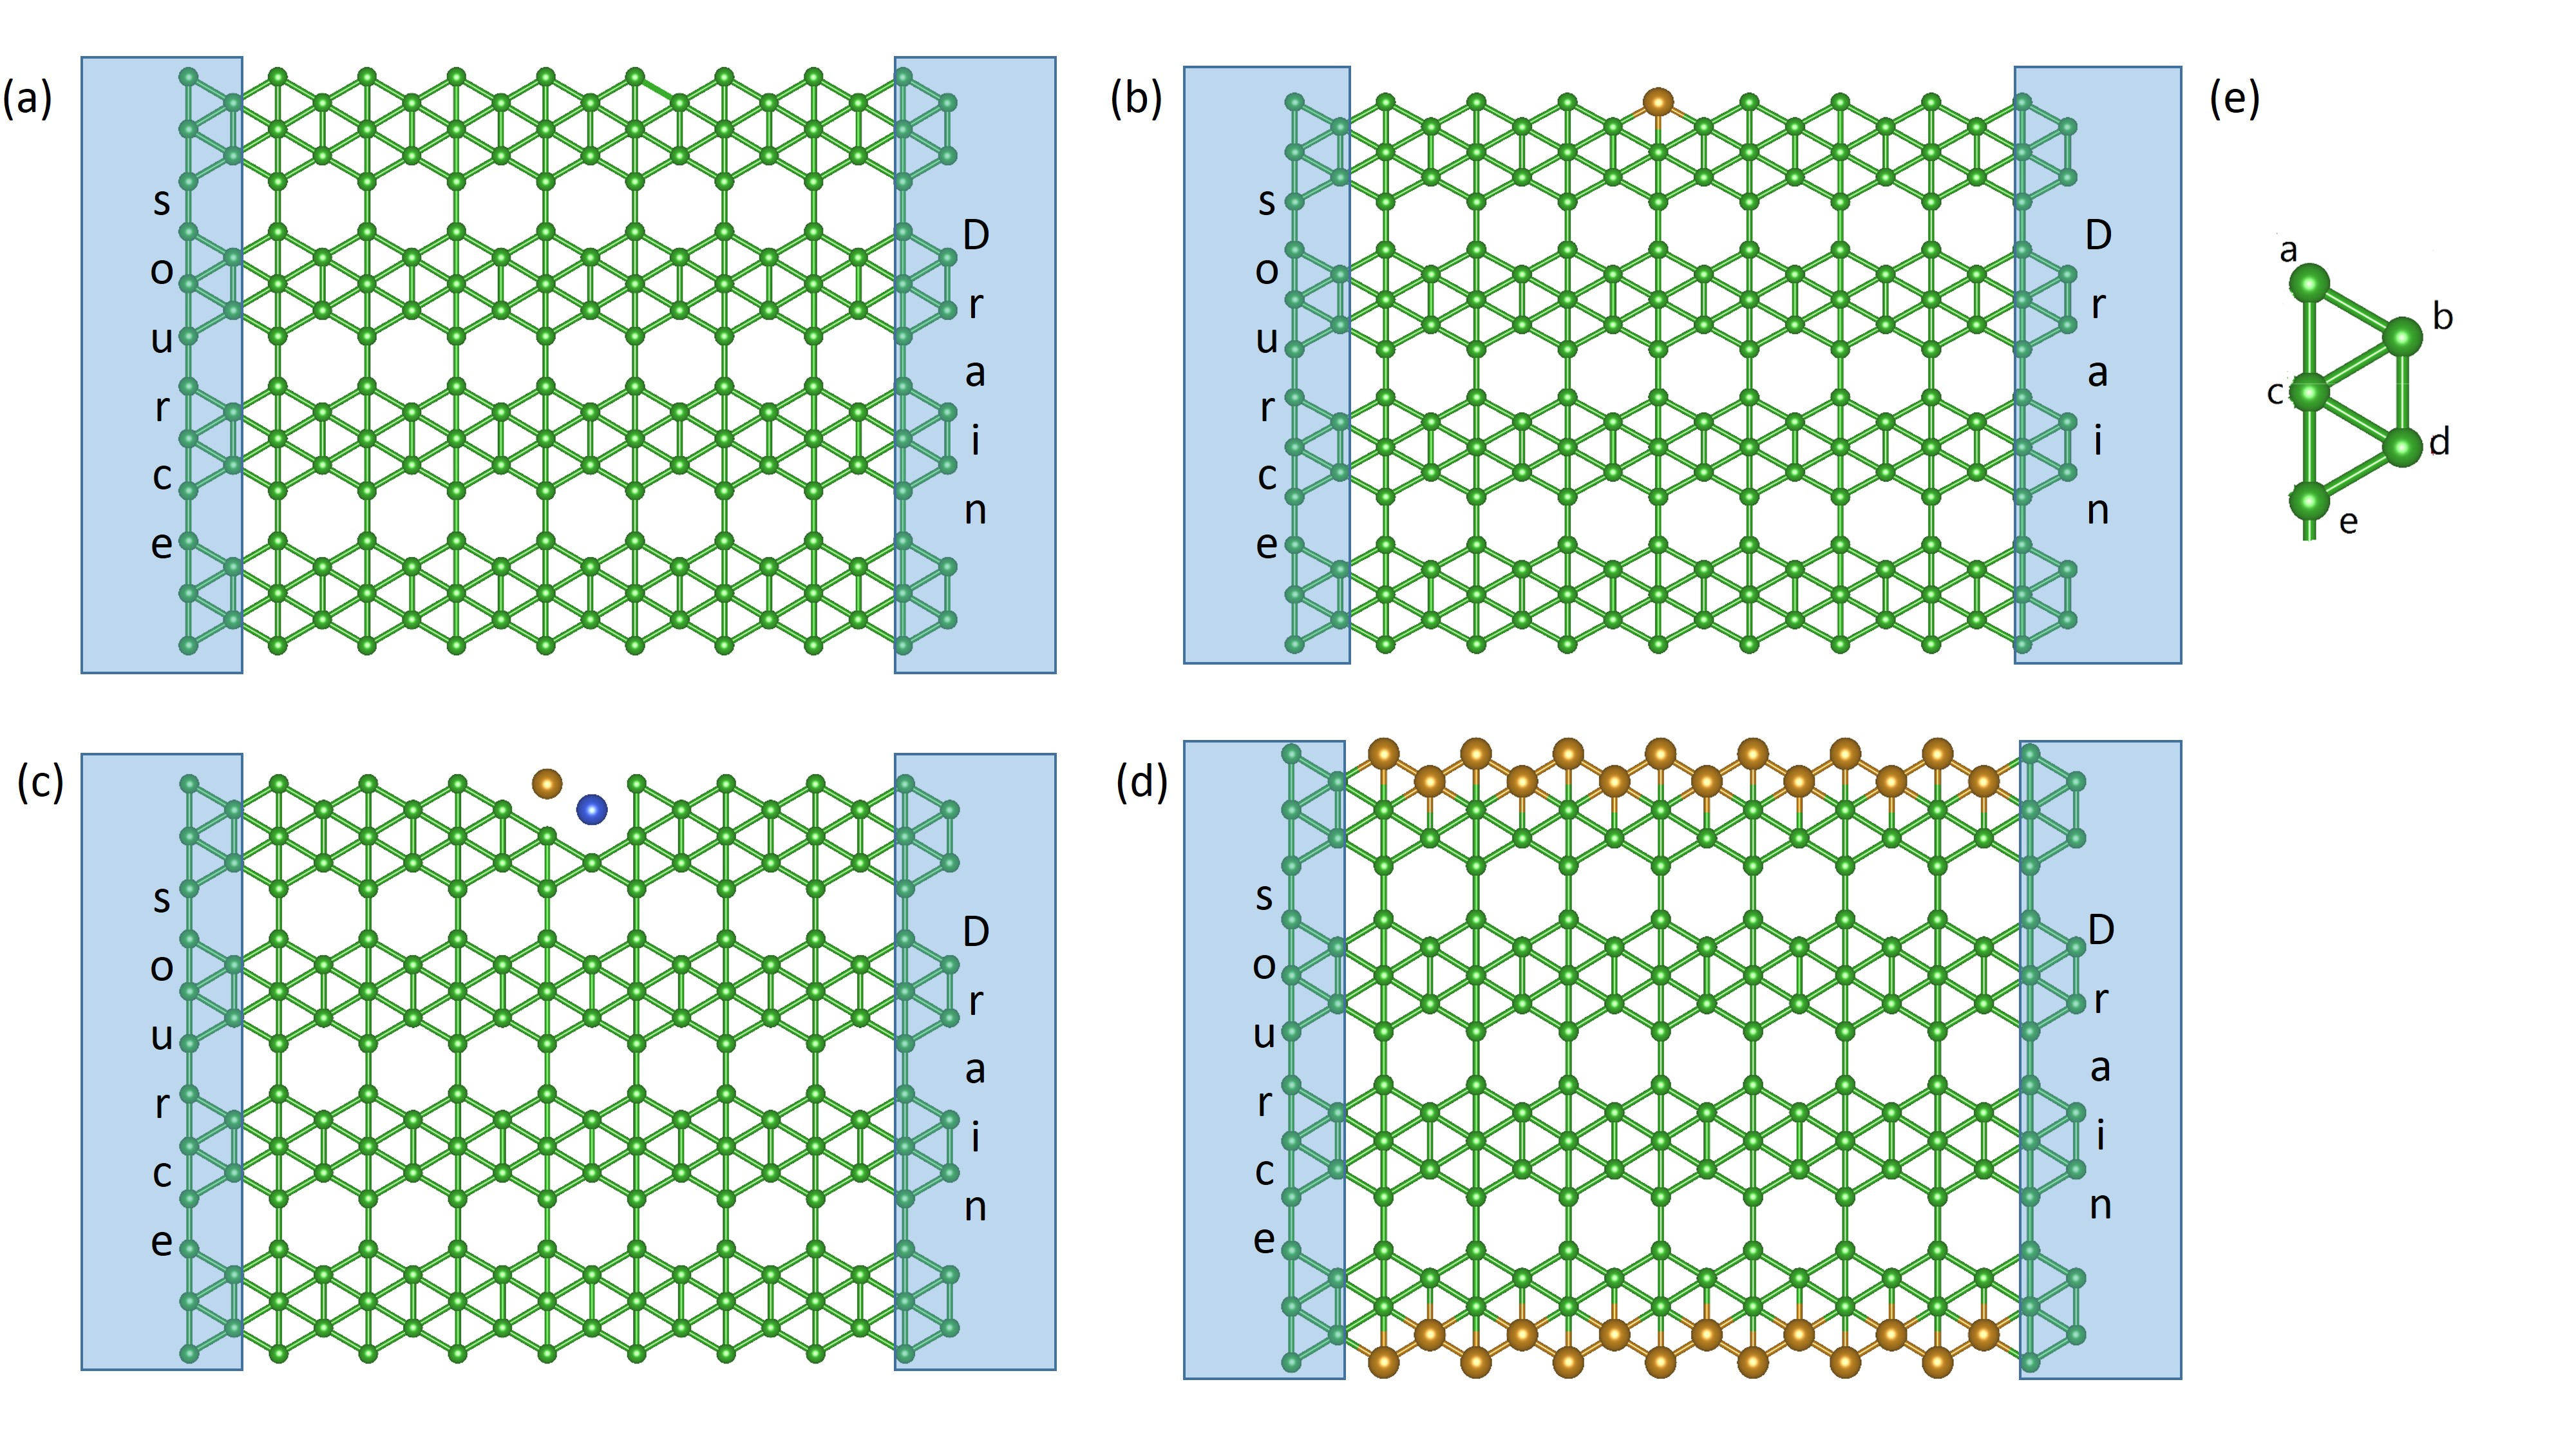
\includegraphics[width=\linewidth]{../figures/borophene_structure(3).JPG}
% 				 \label{fig:borophene}
% 			  \end{figure}
% 		\end{column}
% 	\end{columns}
% \end{frame}
% ---------------------------------------
\begin{frame}{ZBNR with an impurity}
	\begin{columns}[t]
		\begin{column}[t]{0.4\linewidth}
			\begin{itemize}
				\item At certain energies, the impurity leads to conductance dips, accompanied by peaks in LDOS at the nearest neighboring site.
				\item The conductance dips and LDOS peaks can be attributed to quasi-localized states occurring in the vicinity of the impurity.
				% \item The hidden honeycomb lattice in the borophene β12 lattice is responsible for these effects.
			\end{itemize}
		\end{column}
		\begin{column}[t]{0.6\linewidth}
			\begin{figure}[!ht]
				\raggedleft
				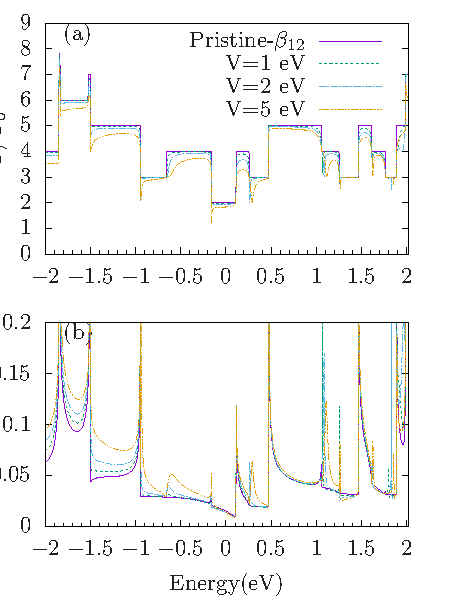
\includegraphics[width=.8\linewidth]{../figures/zigscatter-thesis.eps}
				\label{zigscatter}
			\end{figure}
		\end{column}
	\end{columns}
\end{frame}
% -----------------------------------------------
\begin{frame}{LDOS in ZBNR}
	\begin{itemize}
		\item Increasing the scatterer strength leads to a higher DOS distribution towards the site nearest to the scatterer.
		\item These results confirm the findings from Fig. 2, which showed the impact of scatterers on conductance and local DOS.
		\item The hidden honeycomb lattice in the borophene $\beta_{12}$ lattice is responsible for these effects.
	\end{itemize}
	\begin{figure}[!ht]
		\centering
		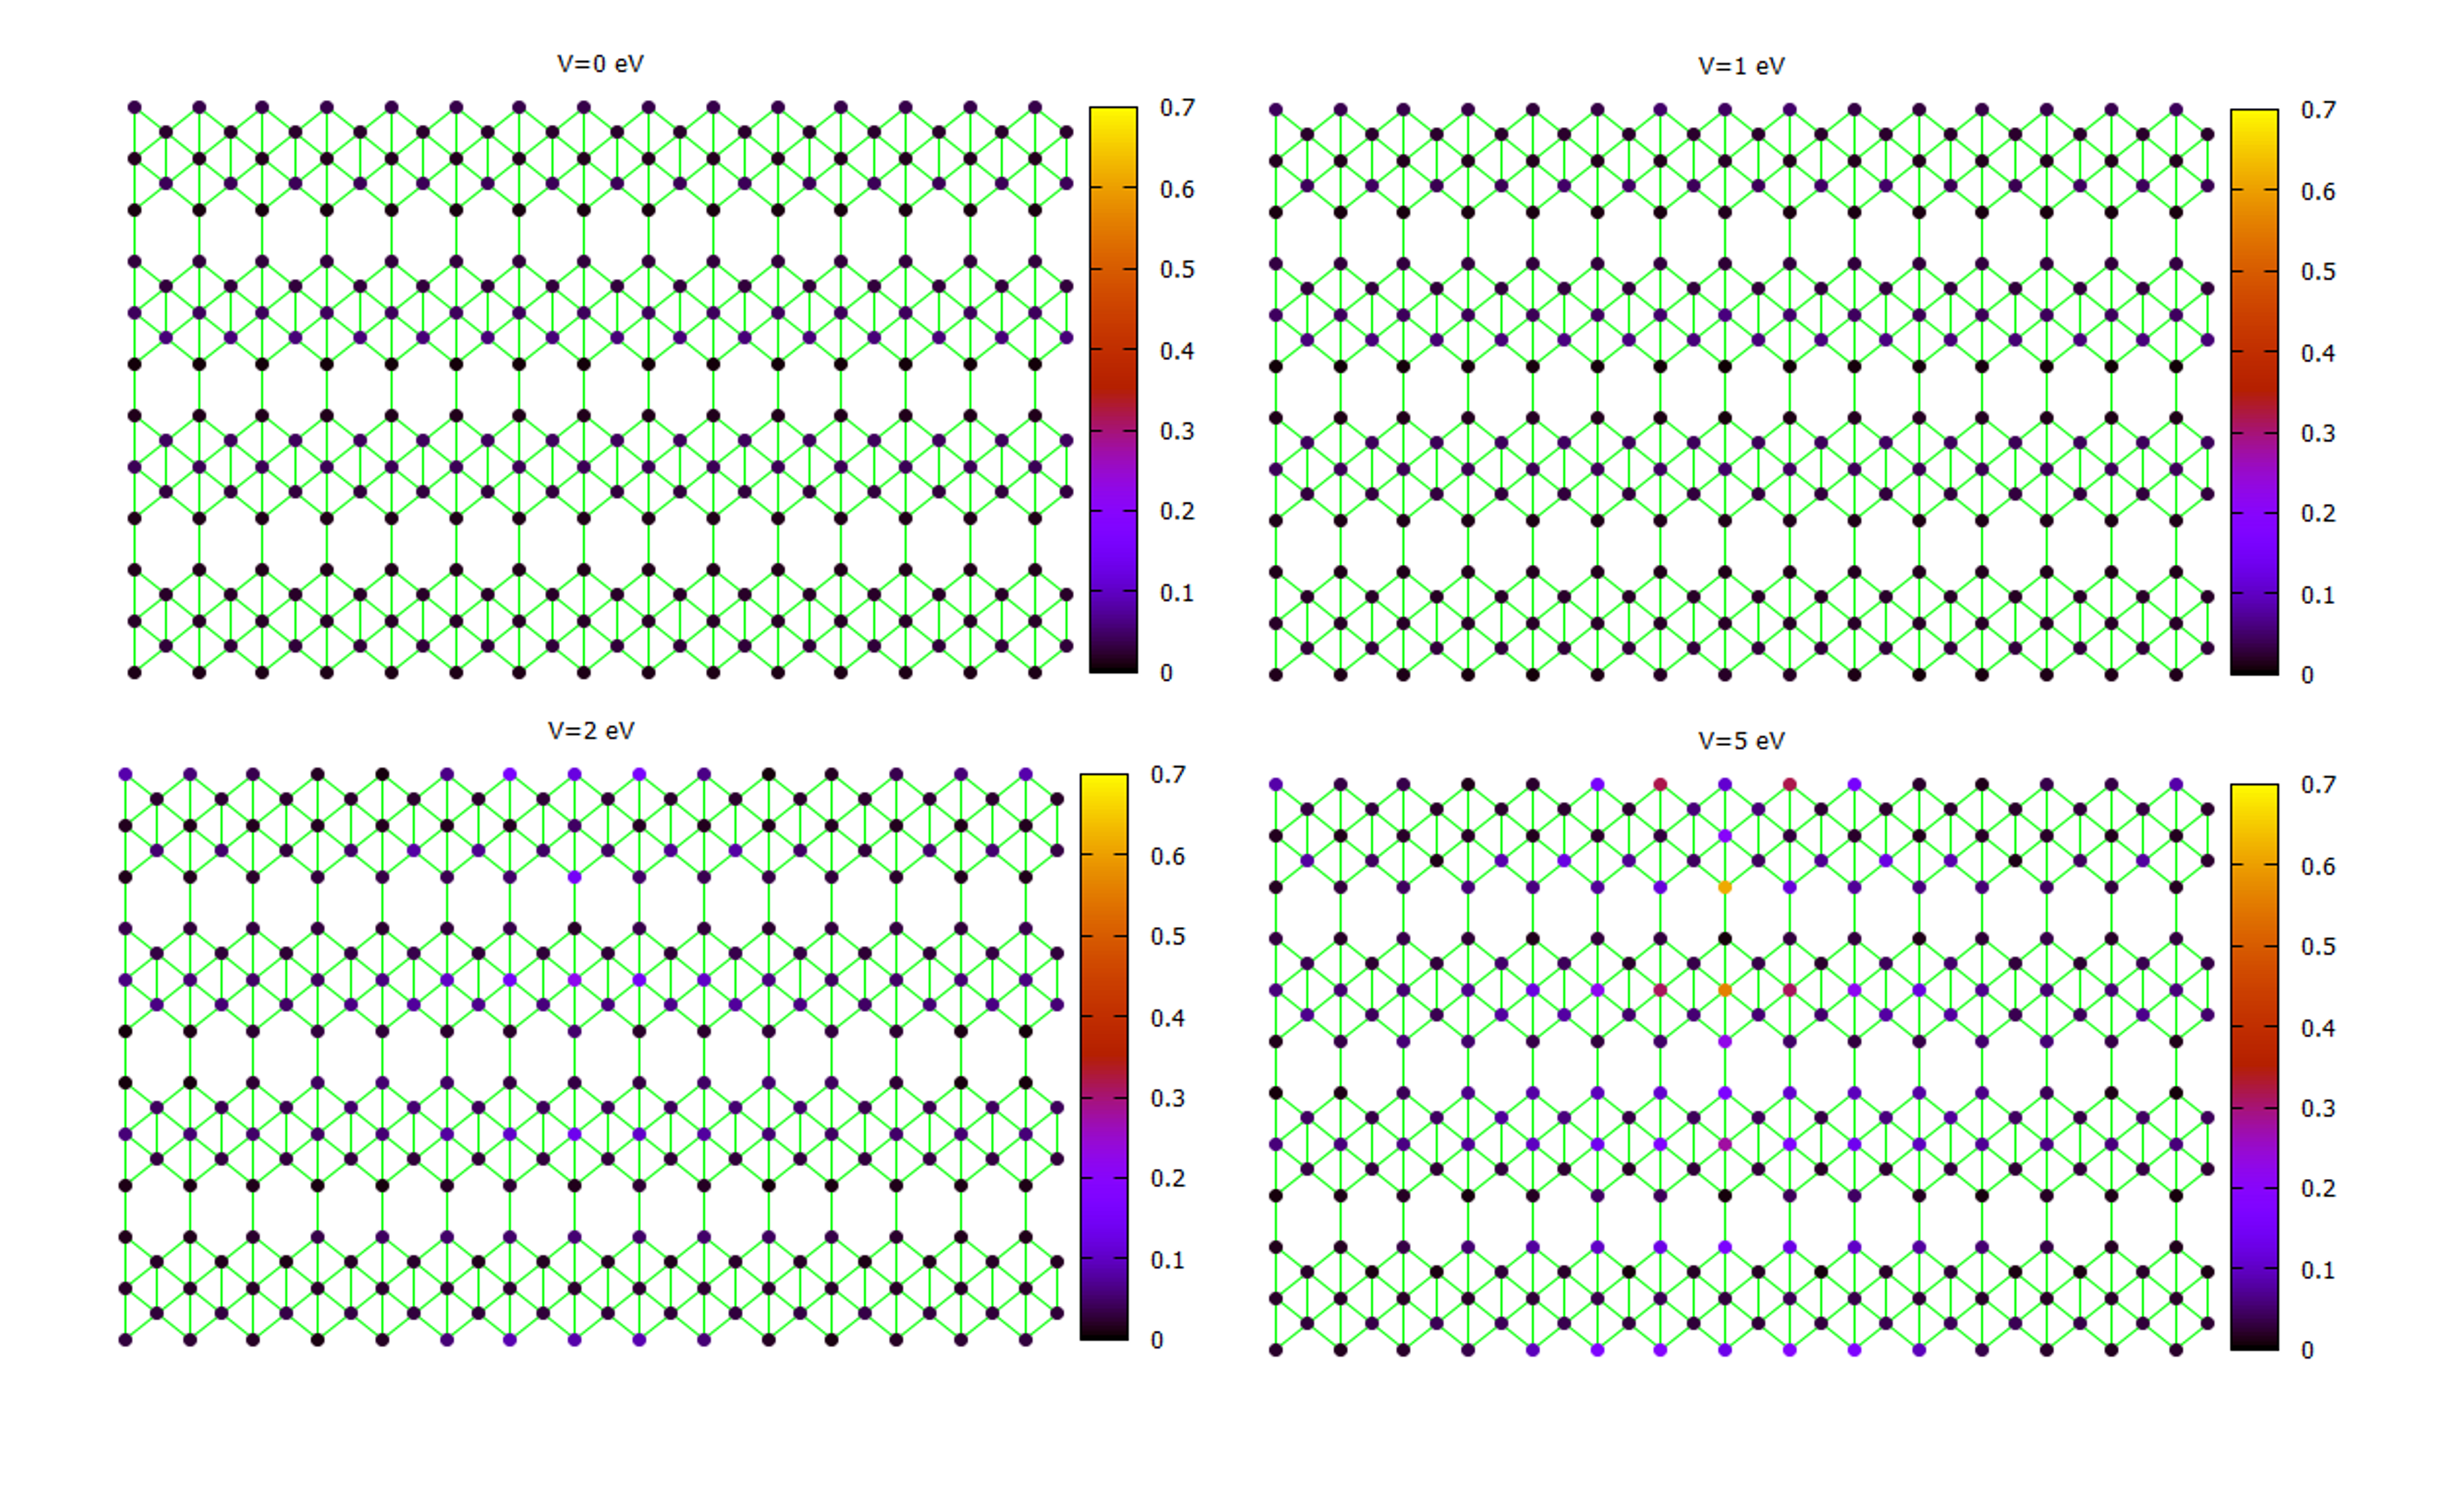
\includegraphics[width=0.7\linewidth]{../figures/Slide1.PNG}
		% \caption{At energy corresponding to the peak of LDOS near the Fermi energy, the spatial electron density of states plotted at the entire site of the zigzag borophene nanoribbon with a scattering site at the upper edge by V=0,1,2,5 in the middle of the nanoribbon.}
		\label{zigCSLDOS}
	  \end{figure}
\end{frame}
% ------------------------------------
\begin{frame}{ABNR with an Impurities}
	\begin{columns}[t]
		\begin{column}[t]{0.5\linewidth}
			\begin{itemize}
				\item  A scatterer on the edge of borophene with an armchair edge has a more significant effect than a scatterer on the edge of borophene with a zigzag edge.
				\item Quasi-localized states can be seen in strong impurities.
				\item 		
			\end{itemize}
		\end{column}
		\begin{column}[t]{0.5\linewidth}
			\begin{figure}[ht]
				\raggedleft
				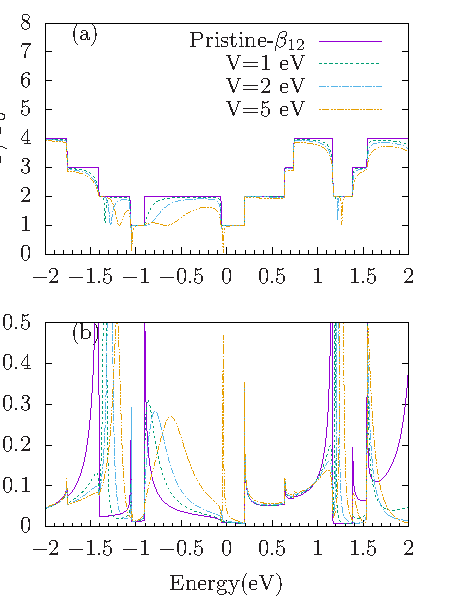
\includegraphics[width=\linewidth]{../figures/armscatter-thesis.eps}
				\label{armscatter}
			\end{figure}
		\end{column}
	\end{columns}
\end{frame}
% -----------------------------------------------
\begin{frame}{LDOS in ANBR with Impurities}
	\begin{columns}
		\begin{column}[t]{.5\linewidth}
			\begin{itemize}
				\item 
			\end{itemize}
		\end{column}
		\begin{column}[t]{.5\linewidth}
			\begin{figure}[!ht]
				\centering
				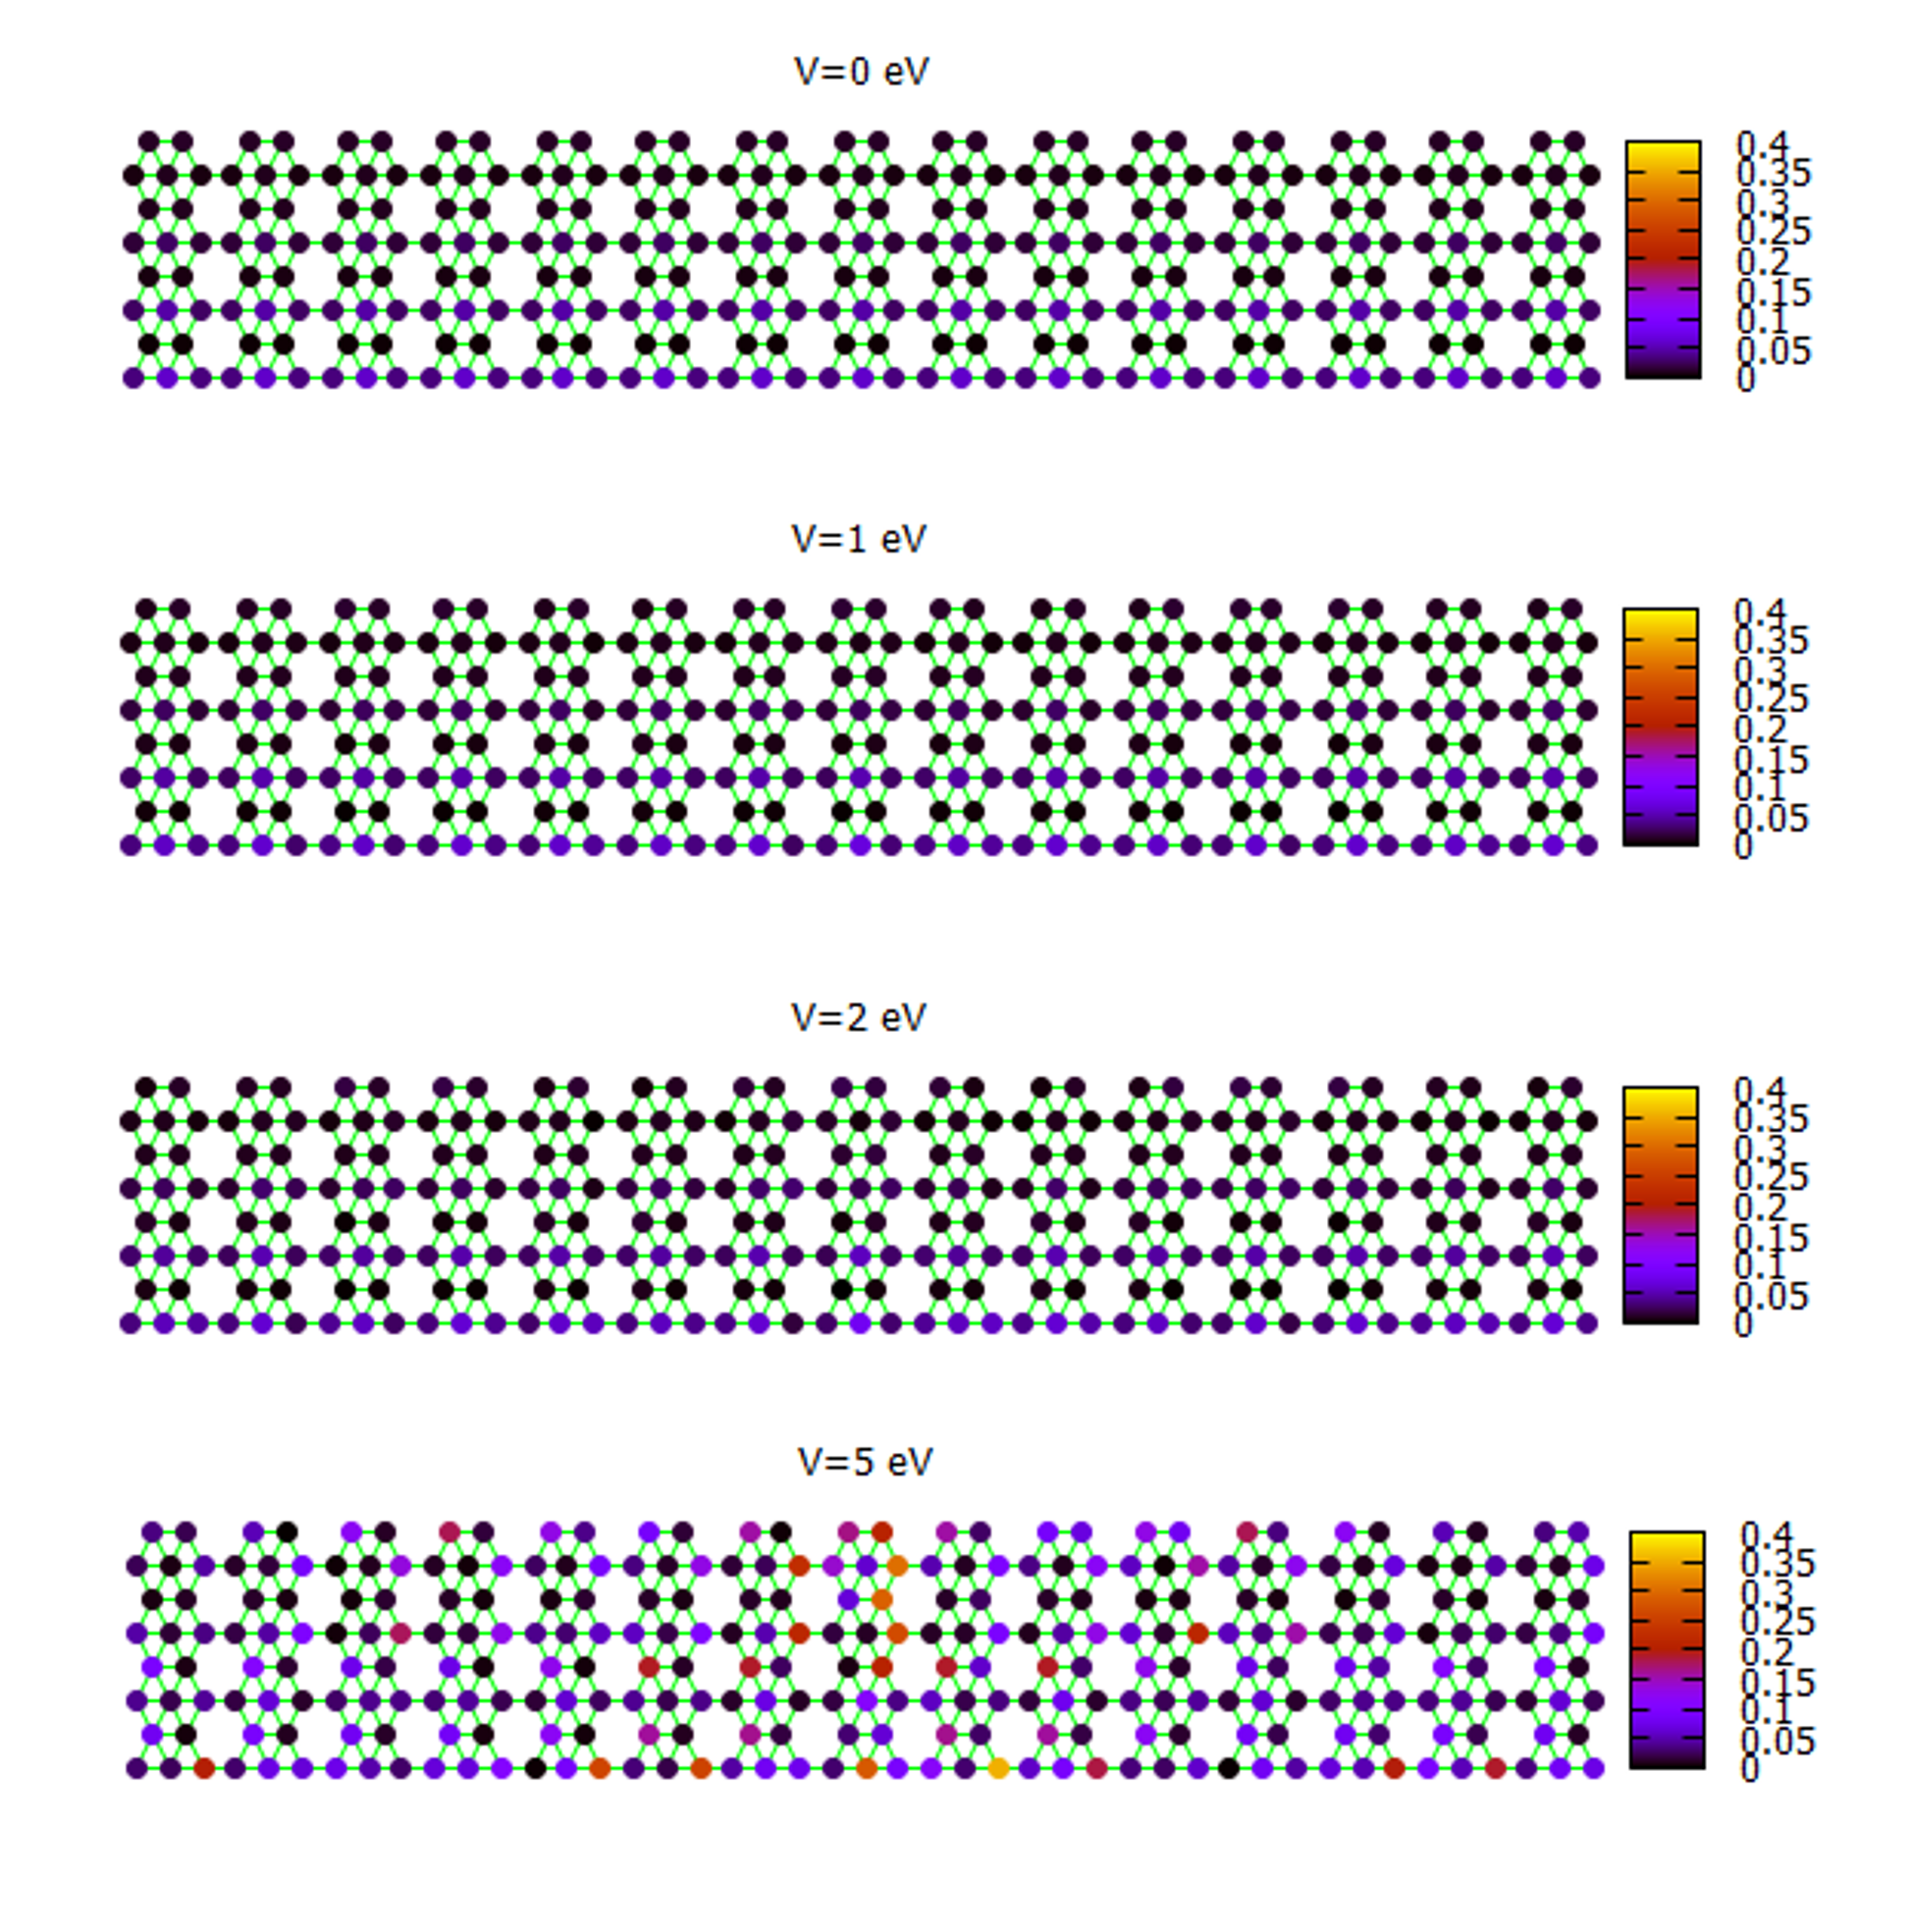
\includegraphics[width=\linewidth]{../figures/Slide3.PNG}
				% \caption{At energy corresponding to the peak of LDOS near the Fermi energy, the spatial electron density of states plotted at the entire site of the armchair borophene nanoribbon with a scattering site at the upper edge by V=0,1,2,5 in the middle of the nanoribbon.}
				\label{armCSLDOS}
			  \end{figure}
		\end{column}
	\end{columns}
\end{frame}
% -----------------------------------------------
\begin{frame}{Edge Vacancies}
	\begin{columns}[t]
		\begin{column}[t]{0.5\linewidth}
			\begin{itemize}
				\item The effect of single-atom edge vacancy and two-atom edge vacancies on the conductance of ABNRs are quite different.
				\item Conductance dips appear at the edges of the bands, different from Van-Hoff singularities of the pristine system.
			\end{itemize}
		\end{column}
		\begin{column}[t]{0.5\linewidth}
			\begin{figure}[ht]
				\raggedleft
				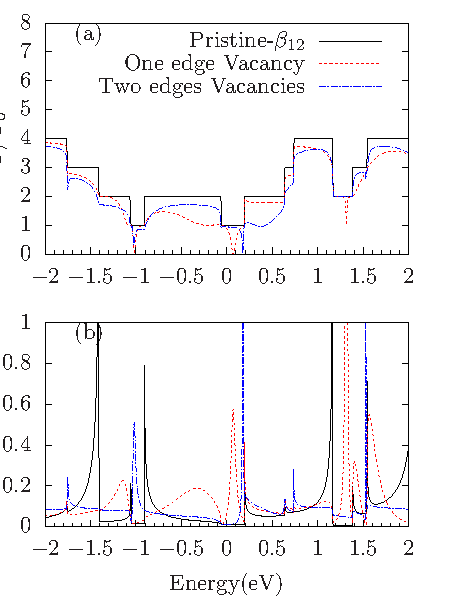
\includegraphics[width=\linewidth]{../figures/armvacancy-thesis.eps}
			\end{figure}
		\end{column}
	\end{columns}
\end{frame}
% -----------------------------------------------
\begin{frame}{Two-Atom Edge Vacancies:}
	\begin{columns}[t]
		\begin{column}[t]{0.5\linewidth}
			\begin{itemize}
				\item A prominent conductance dip appears at the Fermi energy, accompanied by a large LDOS peak.
				\item This is originated from sublattice symmetry breaking, as there is a hidden honeycomb lattice in the $\beta_{12}$ lattice structure.
				\item  The translational symmetry breaking in the presence of a vacancy in the nanoribbon with an armchair edge. 
			\end{itemize}
		\end{column}
		\begin{column}[t]{0.5\linewidth}
			\begin{figure}[!ht]
				\centering
				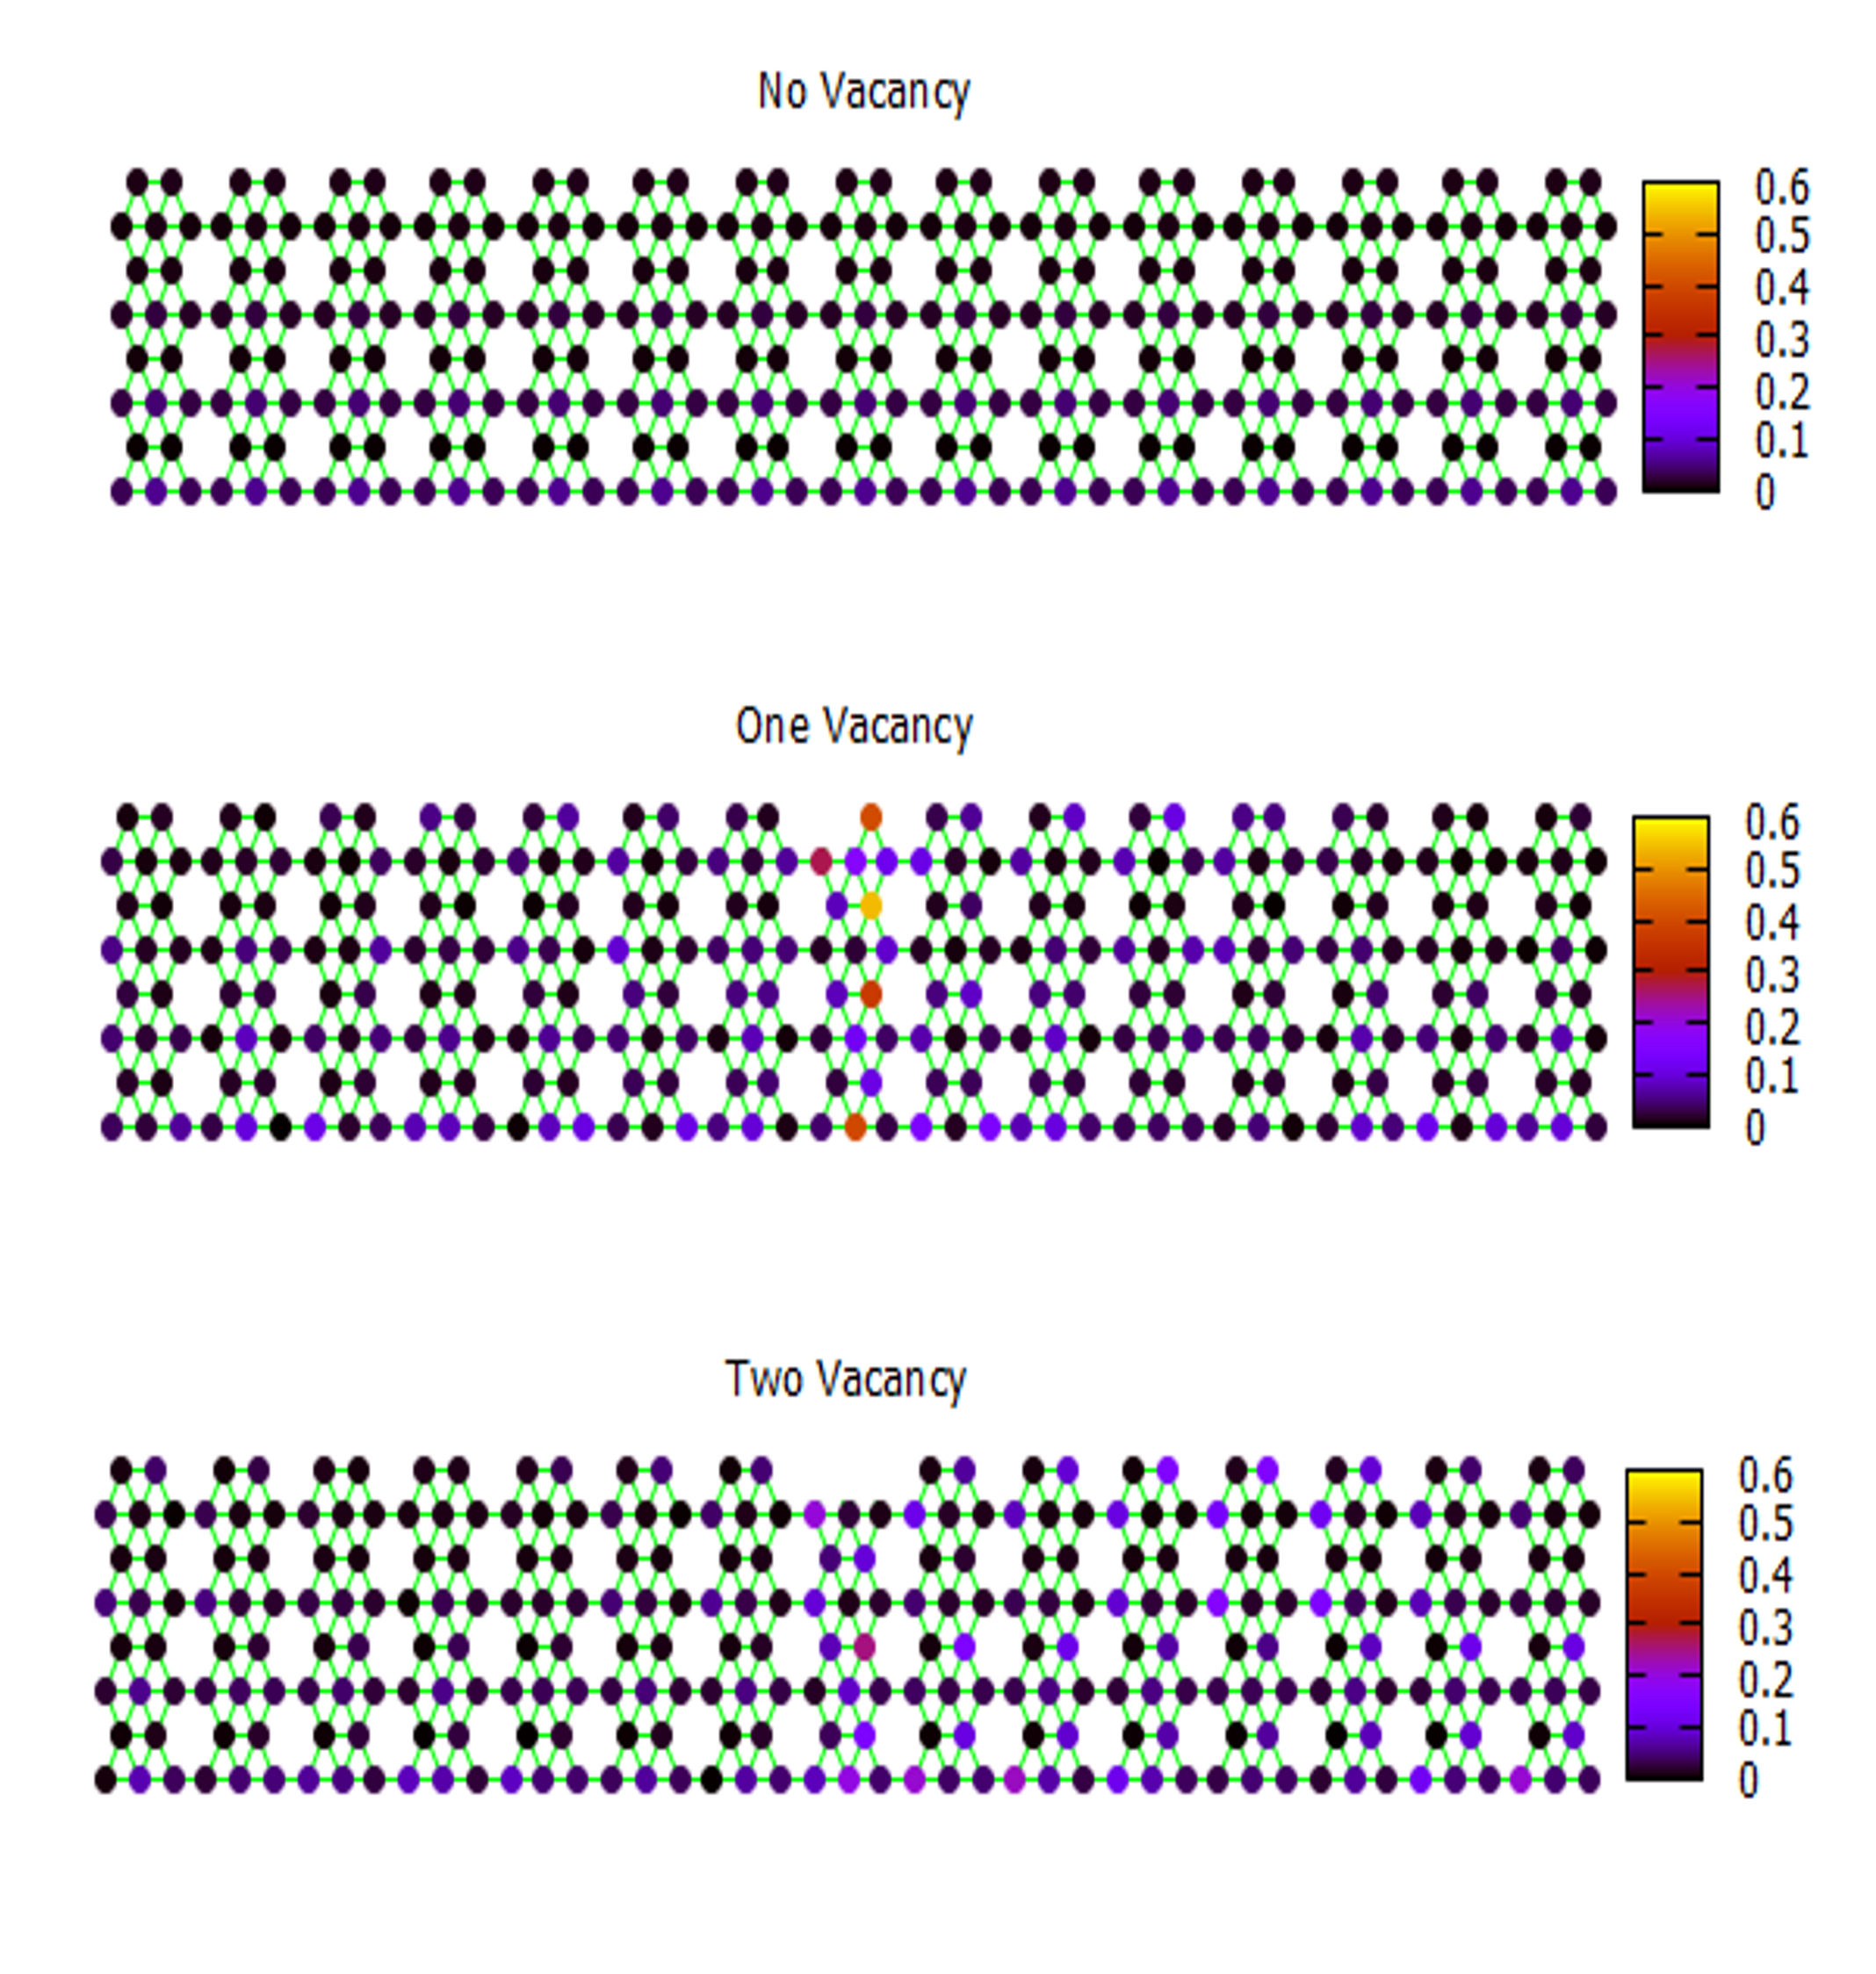
\includegraphics[width=\linewidth]{../figures/Slide5.PNG}
				% \caption{At energy corresponding to the peak of LDOS near the Fermi energy, the spatial electron density of states plotted at the entire site of the armchair borophene nanoribbon with a vacancy site at the upper edge of no vacancy, one vacancy, and two vacancies in the middle of the nanoribbon.}
				\label{armVSLDOS}
			\end{figure}
		\end{column}
	\end{columns}
\end{frame}
% -----------------------------------------------
\begin{frame}{Zigzag Vacancy}
	\begin{columns}[t]
		\begin{column}[t]{0.5\linewidth}
			\begin{itemize}
				\item ZBNRs with a single-atom edge vacancy behave similarly to armchair graphene nanoribbons.
				\item  In the case of two-atom edge vacancies in ZBNRs, a large conductance dip with an equivalent large LDOS appears at the Fermi energy.
				\item 
			\end{itemize}
		\end{column}
		\begin{column}[t]{0.5\linewidth}
			\begin{figure}[ht]
				\raggedleft
				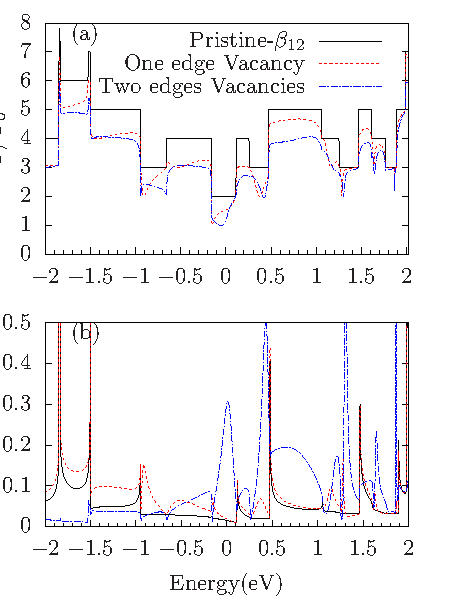
\includegraphics[width=\linewidth]{../figures/zigvacancy-thesis.eps}
				\label{zigvacancy}
			\end{figure}
		\end{column}
	\end{columns}
\end{frame}
% -----------------------------------------------
\begin{frame}{LDOS in ZNBR with Vacancy}
	\begin{itemize}
		\item  In the case of two-atom edge vacancies in ZBNRs, a large conductance dip with an equivalent large LDOS appears at the Fermi energy. 
		\item The large conductance dip and LDOS peak can be explained by the breaking of sublattice symmetry due to the presence of a middle atom in the unit cell at the edge.
		\item  This behavior is similar to that observed in armchair borophene nanoribbons (ABNRs) but contradictory to that of graphene nanoribbons (GNRs).
	\end{itemize}
	\begin{figure}[!ht]
		\centering
		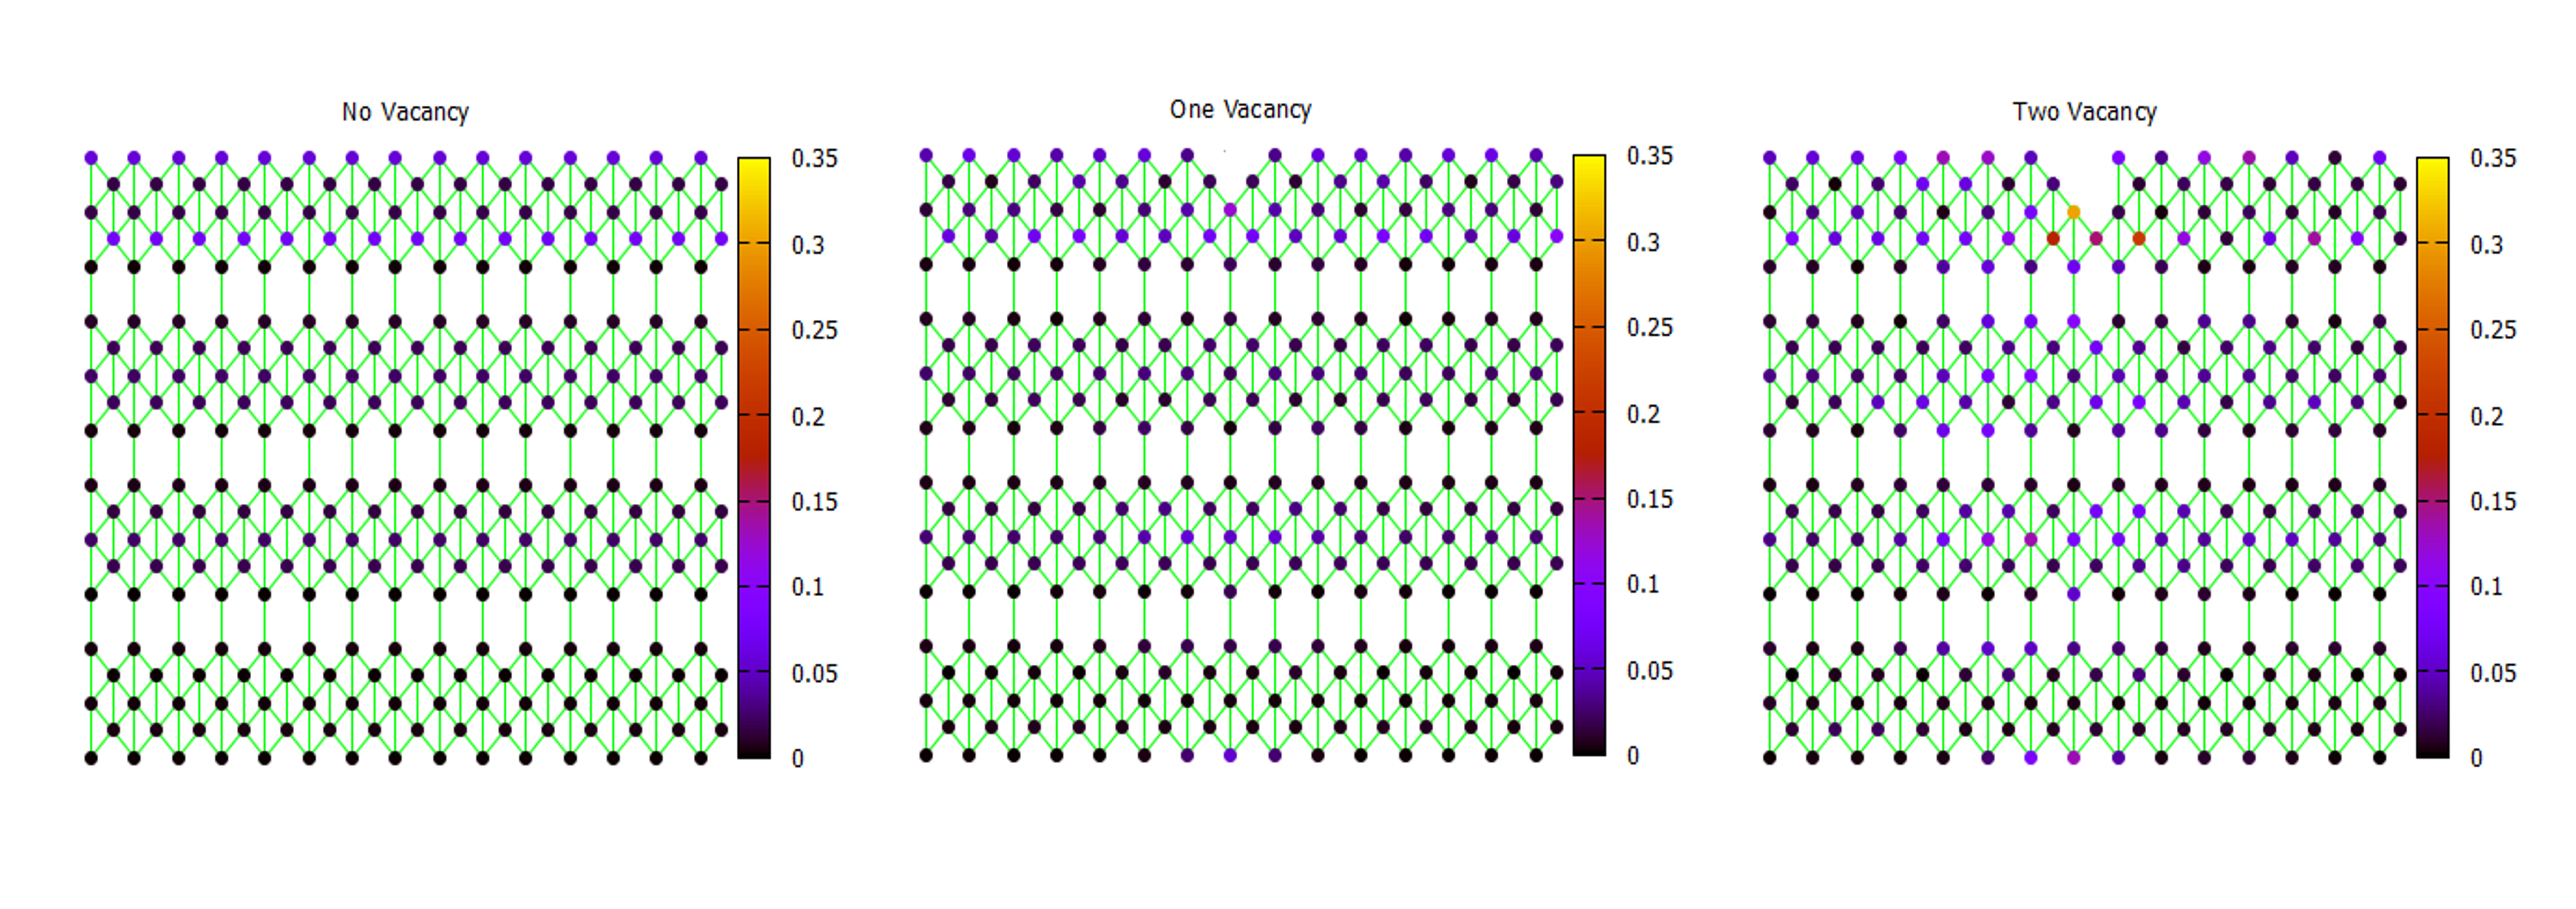
\includegraphics[width=1\linewidth]{../figures/Slide4.PNG}
		% \caption{At energy corresponding to the peak of LDOS near the Fermi energy, the spatial electron density of states plotted at the entire site of 
		% the zigzag borophene nanoribbon with a vacancy site at the upper edge of no vacancy, one vacancy, and two vacancies in the middle of the nanoribbon.}
		\label{zigVSLDOS}
	\end{figure}
\end{frame}
% end of subsection
% -----------------------------------------------
\subsection{Anderson Localization}
% -----------------------------------------------
\begin{frame}{Anderson Localization: Wave Interference and Disorder}
	\begin{itemize}
		\item Anderson localization is a phenomenon resulting from the interference of propagating waves from multiple paths, observed in various wave systems.
		\item Understanding Anderson localization requires controlling factors such as interparticle interactions, dimensionality, time-reversal symmetry, and the microscopic nature of the disorder.
		\item Ultracold atom systems provide an appropriate and controllable platform for studying Anderson localization.
	\end{itemize}
\end{frame}
% -----------------------------------------------
\begin{frame}{Anderson Localization in Solid-State Physics:}
	\begin{itemize}
		\item Anderson localization predicts that an electron may be immobilized in a disordered lattice.
		\item In a periodic quantum system, single-particle eigenstates are extended (delocalized) throughout space (Bloch theorem).
		\item Static disorder breaks the crystal and Hamiltonian translational symmetry, increasing the probability of exponentially localized eigenstates.
		\item Greater disorder leads to more localized eigenstates, and in some cases, Anderson transition occurs, transforming all extended states into localized states.
	\end{itemize}
\end{frame}
% -----------------------------------------------
\begin{frame}{Extended vs. Localized Eigenstates:}
	\begin{itemize}
		\item Extended states give rise to a mean-squared displacement that grows with time for long times, while localized states do not.
		\item The presence or absence of extended states determines the possibility of particle transport over macroscopic length scales.
		\item Anderson localization can explain transition phenomena, including metal-insulator transitions in semiconductors.
		\item The potential strength of the impurities is chosen randomly from the range [-Vd, Vd], where Vd is the maximum disorder strength.
		\item Impurities are distributed only along the upper and lower edges of the nanoribbons.
	\end{itemize}
\end{frame}
% -----------------------------------------------
\begin{frame}{Weak disorder}
	\begin{itemize}
	\item Very weak disorder potentials reduce conductance but cannot cause Anderson localization in ZBNRs.
	\item As the potential strength increases, localization occurs around $-0.5\; eV$ when $V_d = 2\; eV$.
	\item The localization length in ABNRs is much shorter than the localization length observed in ZBNRs.
	\item 
	\end{itemize}
	\begin{figure}[ht]
		\centering
		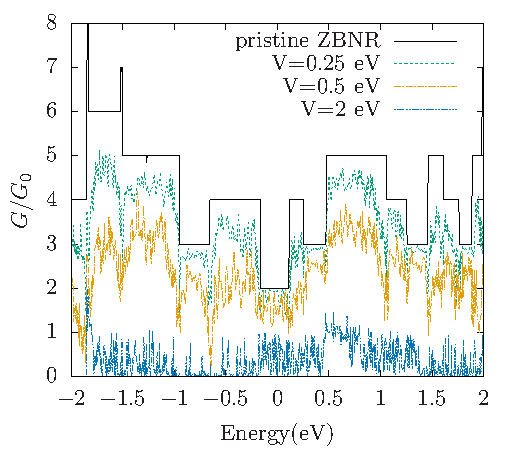
\includegraphics[width=0.45\linewidth]{../figures/zigzagdisorder-thesis.eps}
		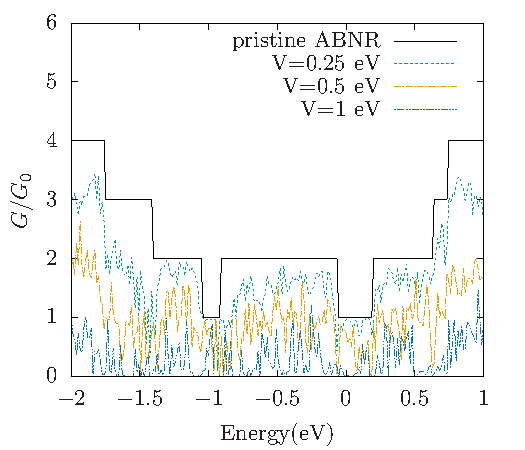
\includegraphics[width=0.45\linewidth]{../figures/armdisorder-thesis.eps}
	\end{figure}
\end{frame}
% -----------------------------------------------
% \begin{frame}{armdisorder}
% 	\begin{columns}[t]
% 		\begin{column}[t]{.5\linewidth}
% 			\begin{itemize}
% 				\item The localization length in ABNRs is much shorter than the localization length observed in ZBNRs.
% 				\item 
% 			\end{itemize}
% 		\end{column}
% 		\begin{column}[t]{0.5\linewidth}
% 			\begin{figure}[ht]
% 				\raggedleft
% 				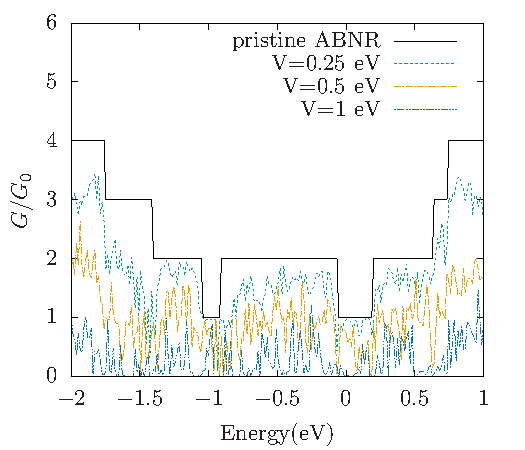
\includegraphics[width=\linewidth]{../figures/armdisorder-thesis.eps}
% 			\end{figure}
% 		\end{column}
% 	\end{columns}
% \end{frame}
% -----------------------------------------------
\begin{frame}{Localization length}
	\begin{itemize}
		\item The localization length is the length at which extended Bloch eigenstates change into localized states, resulting in zero conductance.
		\item With increasing ribbon length and a potential strength of $2\;eV$ at the edges, the conductance decreases exponentially.
		\item An increase in the number of conductance channels is observed when the widths of ABNRs increase, similar to the trend observed for ZBNRs.
		% \item The physical reason behind the greater impact of weak disorder on the conductance of ABNRs compared to ZBNRs can be understood by considering the higher speed of the electron group velocity in ZBNRs compared to ABNRs in the Fermi energy range.
	\end{itemize}
	\begin{figure}[ht]
		\raggedleft
		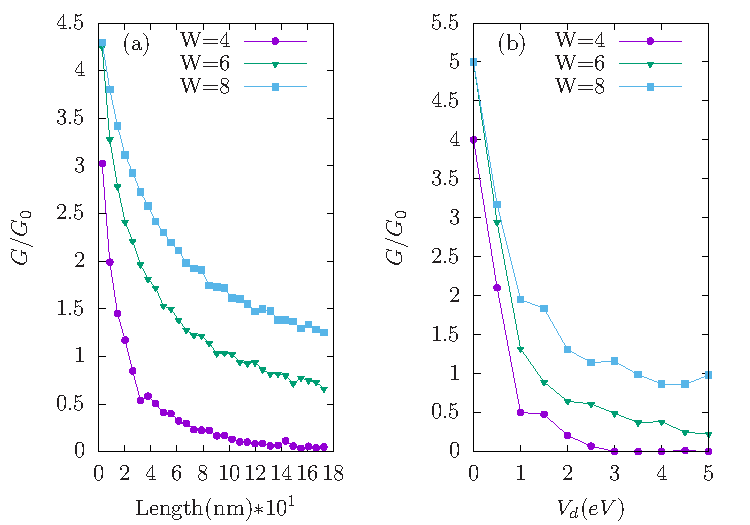
\includegraphics[width=0.5\linewidth]{../figures/zigzag-width-strangth-thesis.eps}
		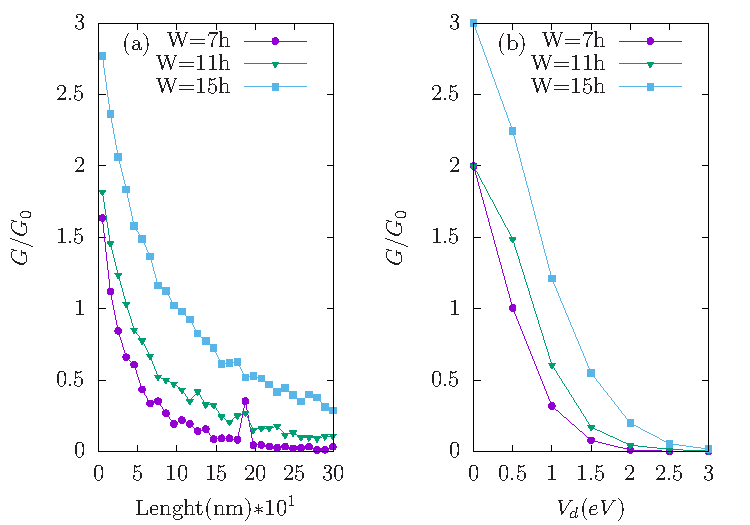
\includegraphics[width=0.5\linewidth]{../figures/armchair-width-strangth-thesis.eps}
	\end{figure}
\end{frame}
% -----------------------------------------------
% \begin{frame}{zigzag-width-strangth}
% 	\begin{columns}[t]
% 		\begin{column}[t]{0.4\linewidth}
% 			\begin{itemize}
% 				\item The localization length is the length at which extended Bloch eigenstates change into localized states, resulting in zero conductance.
% 				\item With increasing ribbon length and a potential strength of $2\;eV$ at the edges, the conductance decreases exponentially.
% 			\end{itemize}
% 		\end{column}
% 		\begin{column}[t]{0.6\linewidth}
% 			\begin{figure}[ht]
% 				\raggedleft
% 				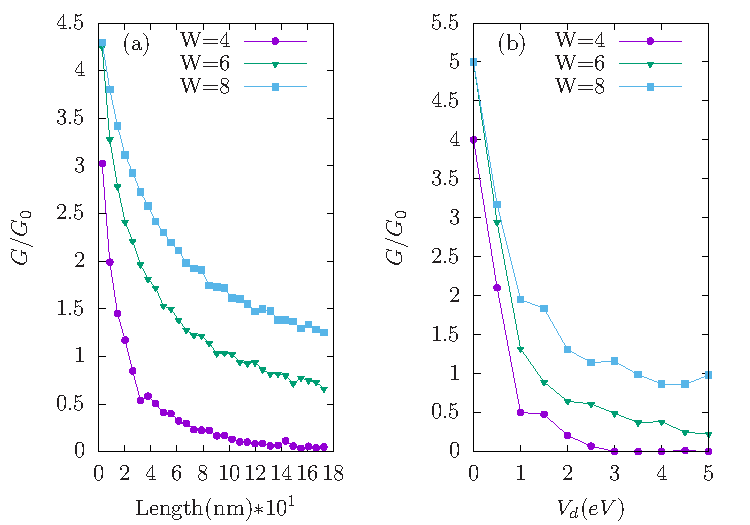
\includegraphics[width=\linewidth]{../figures/zigzag-width-strangth-thesis.eps}
% 			\end{figure}
% 		\end{column}
% 	\end{columns}
% \end{frame}
% -----------------------------------------------
% \begin{frame}{armchair-width-strangth}
% 	\begin{columns}[t]
% 		\begin{column}[t]{0.4\linewidth}
			
% 		\end{column}
% 		\begin{column}[t]{0.6\linewidth}
% 			\begin{figure}[ht]
% 				\raggedleft
% 				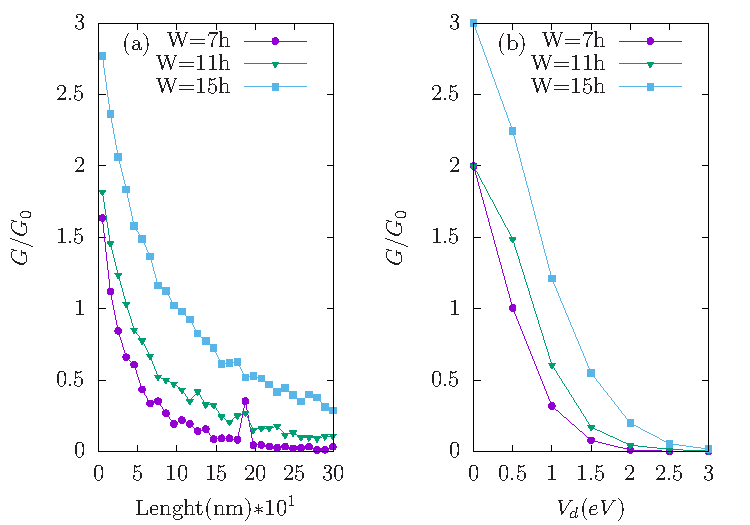
\includegraphics[width=\linewidth]{../figures/armchair-width-strangth-thesis.eps}
% 			\end{figure}
% 		\end{column}
% 	\end{columns}
% \end{frame}

% end of section

% =================== second articles ==========
\section{Spin Conductance}
% ----------------------------------------------
\subsection{Spin Valve}
% ----------------------------------------------
\begin{frame}{Spin Rotation and Conductance Changes in Spin Valves with Ferromagnetic Leads}
	\begin{itemize}
		\item Applying an in-plane exchange magnetic field causes the spin-polarized Hamiltonian to not commute with the spin operator S, implying that the electron spin is no longer a constant of motion in the system.
		\item As a result, the spin state may change along the transport direction due to the interaction between the electron spin and the in-plane exchange magnetic field, leading to spin rotation.
		\item When a magnetic field is applied to the leads due to the presence of a ferromagnetic insulating substrate, an out-of-plane magnetic field is introduced into the spin valves.
		\item A careful analysis of these conductance changes is crucial for understanding their origin and designing applicable spin valves to exploit their full potential.
	\end{itemize}
\end{frame}
% ----------------------------------------------
\begin{frame}{Changes in Conductance Plateaus}
	\begin{itemize}
		\item As a result of changing the magnetic properties of the leads from the non-magnetized case to the magnetized one, there is a change in the number and width of the conductance plateaus.
		\item With increasing magnetization, deviation from the step-like structure in the conductance diagram is observed.
		\item This deviation is due to the separation of energy levels in the electrodes and energy subband parity conservation.
		\item In borophene, the presence of an additional atom in the center of the hexagon leads to an indentation of the energy levels due to exchange interaction, resulting in a greater diversity of subband spacing and wider variation in plateau widths in the conductance diagram.
	\end{itemize}
\end{frame}
% ---------------------------------------------
\begin{frame}{Spin Conductance}
	\begin{columns}[t]
		\begin{column}[t]{0.5\linewidth}
			\begin{figure}
				\raggedleft
				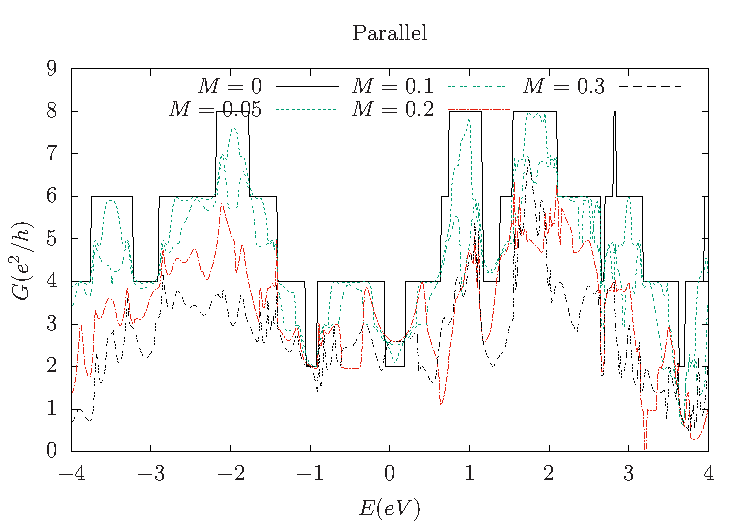
\includegraphics[width=0.88\linewidth]{../figures/armchair-parallel-conductance-revise-thesis.eps}\\
				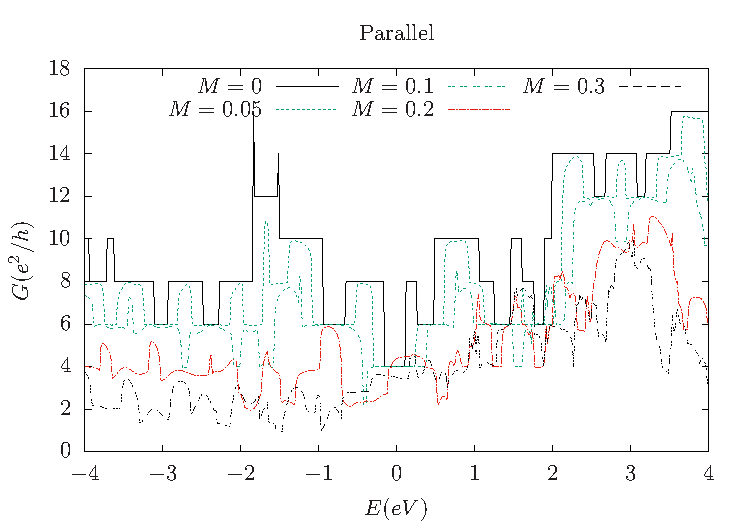
\includegraphics[width=0.88\linewidth]{../figures/zigzag-parallel-conductance-revise-thesis.eps}
			  \end{figure}
		\end{column}
		\begin{column}[t]{0.5\linewidth}
			\begin{figure}
				\raggedleft
				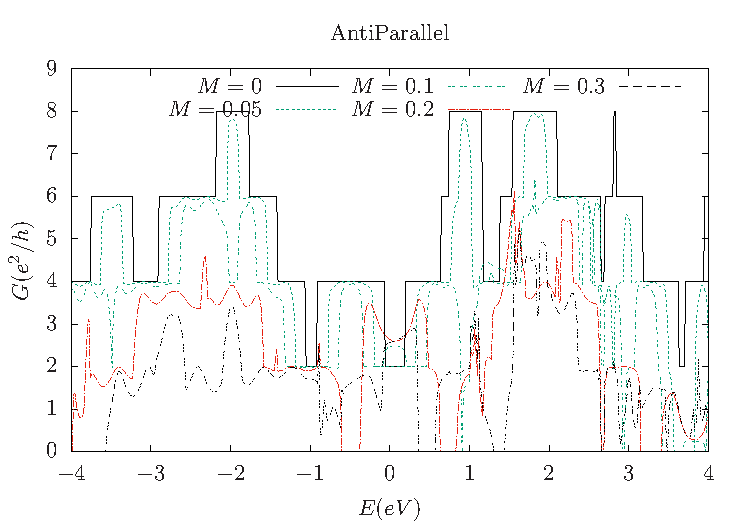
\includegraphics[width=0.88\linewidth]{../figures/armchair-antiparallel-conductance-revise-thesis.eps}\\
				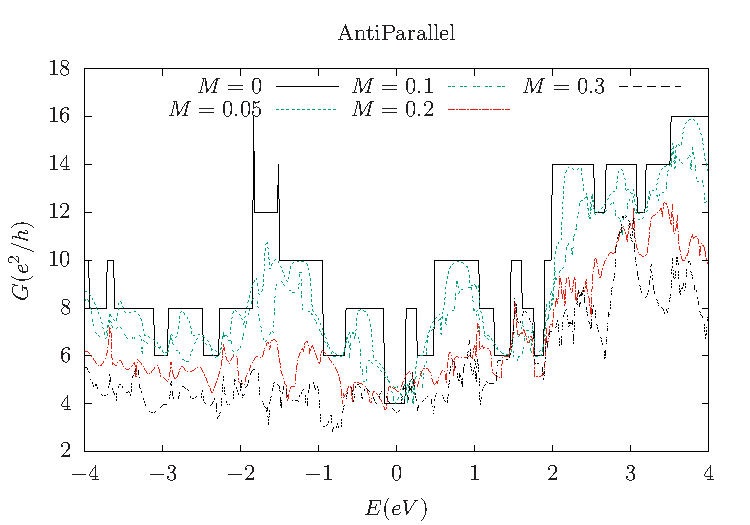
\includegraphics[width=0.88\linewidth]{../figures/zigzag-antiparallel-conductance-revise-thesis.eps}
			  \end{figure}
		\end{column}
	\end{columns}
\end{frame}
% ----------------------------------------------
% \begin{frame}{parallel-conductance}
% 	\begin{columns}[t]
% 		\begin{column}[t]{0.3\linewidth}
% 			1. First\\
% 			2. secend\\
% 			3. thired\\
% 			5. forth
% 		\end{column}
% 		\begin{column}[t]{0.7\linewidth}
% 			\begin{figure}
% 				\raggedleft
% 				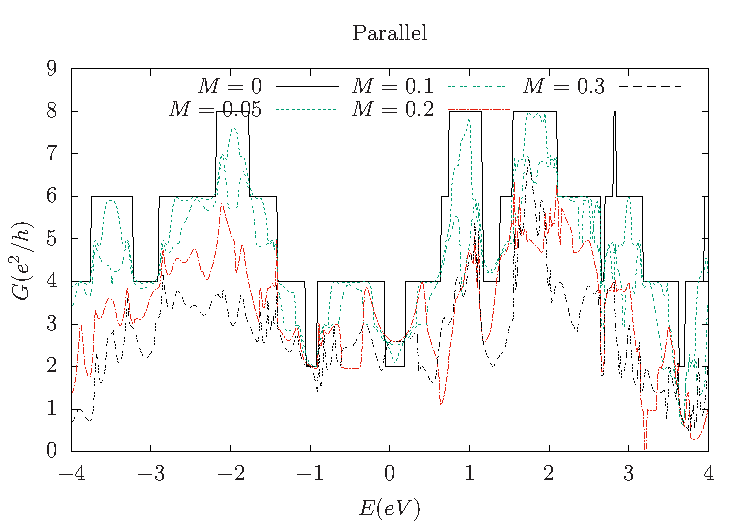
\includegraphics[width=0.6\linewidth]{../figures/armchair-parallel-conductance-revise-thesis.eps}\\
% 				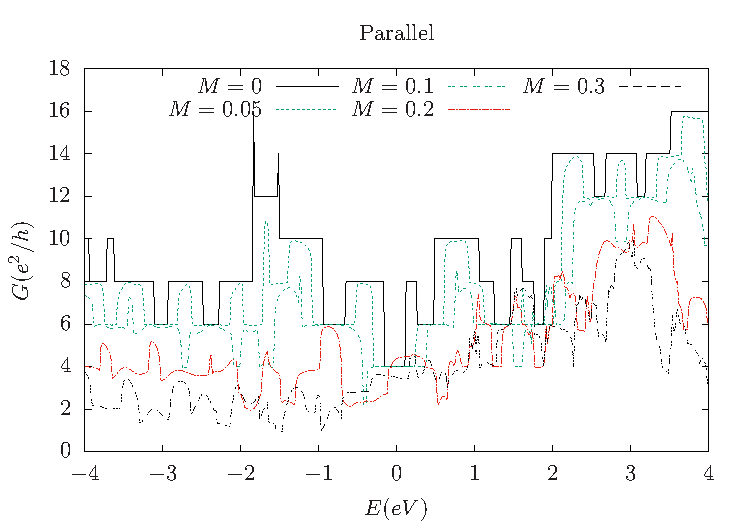
\includegraphics[width=0.6\linewidth]{../figures/zigzag-parallel-conductance-revise-thesis.eps}
% 			  \end{figure}
% 		\end{column}
% 	\end{columns}
% \end{frame}
% -------------------------------------------
\begin{frame}{Conductance Fluctuations in Magnetized Leads}
	\begin{itemize}
		\item In magnetized leads, conductance steps or fluctuations with values smaller than $G_0$ ($G_0 = e^2/h$) can be observed in each configuration (parallel (P) and anti-parallel (AP)).
		\item This phenomenon is caused by the mismatch between the parity of the subbands in the channel and the parity of the subbands in the electrodes.
		\item The tunnel value is less than one $G_0$ in the magnetized case, in contrast to the non-magnetic case.
		\item In addition to the number of subbands in the energy window, the parity of the subbands is also crucial in tunneling and electron transmission processes.
		\item This subsequently causes plateaus with odd values (semi-metallic properties) or semi-integer values.
	\end{itemize}
\end{frame}
% -----------------------------------------------
\begin{frame}{Two channel}
	\begin{figure}[!ht]
		\centering
		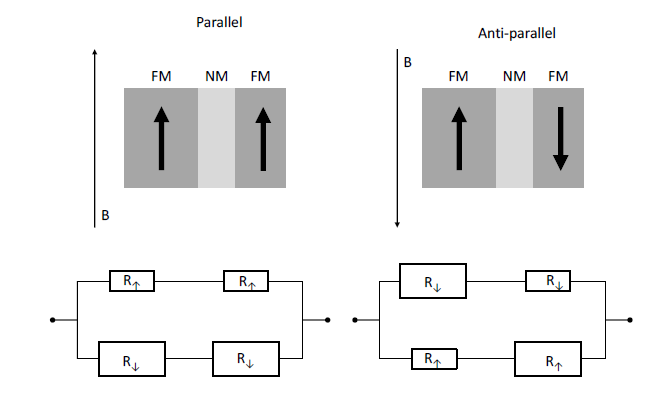
\includegraphics[width=\linewidth]{../figures/twochannelmodel.png}
		\label{fig:twochannelmodel}
	\end{figure}
\end{frame}
% ----------------------------------------------
% end of subsection
% ---------------------------------------------
\subsection{Parity Effect}
% ----------------------------------------------
\begin{frame}{Bands Structure}
	\begin{figure}[ht]
		\centering
		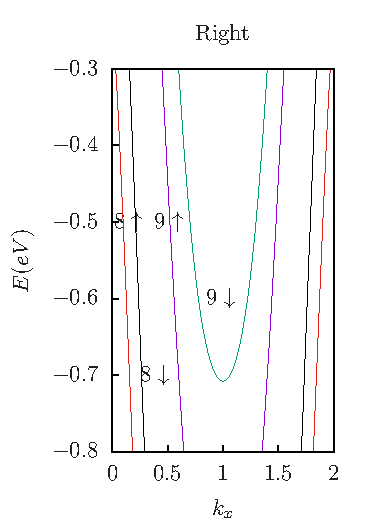
\includegraphics[width=0.33\linewidth]{../figures/Rborophene_band-revised-thesis.eps}
		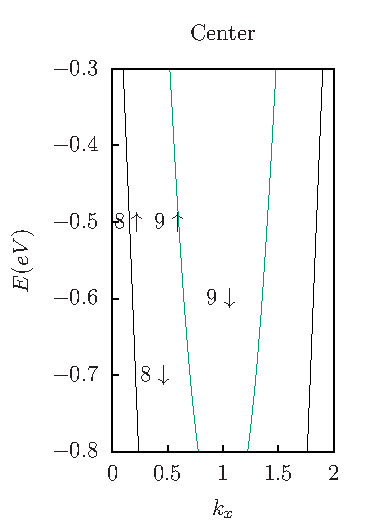
\includegraphics[width=0.33\linewidth]{../figures/Cborophene_band-revised-thesis.eps}
		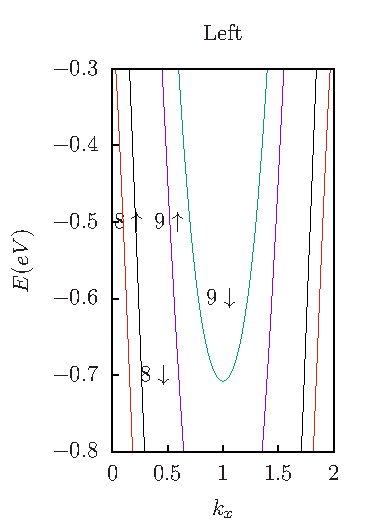
\includegraphics[width=0.33\linewidth]{../figures/Lborophene_band-revised-thesis.eps}
	\end{figure}
	\begin{itemize}
		\item The subbands have parity symmetry due to the symmetric structure of the Hk matrix, with even-parity subbands (0, 2, 4, ...) and odd-parity subbands (1, 3, 5, ...).
	\end{itemize}
\end{frame}
% -----------------------------------------------
\begin{frame}
	\begin{itemize}
		\item In the anti-parallel (AP) configuration, the order of the split subbands is reversed in the opposite electrode.
		\item Due to the renumbering of parity, subbands with the same number in two electrodes with opposite magnetizations will have opposite parity.
		\item An even-parity electron at the left electrode will not yield an odd-parity electron at the right electrode during the tunneling process, leading to zero conductance, even in the absence of a band gap in that energy range.
	\end{itemize}
	\begin{figure}[ht]
		\centering
		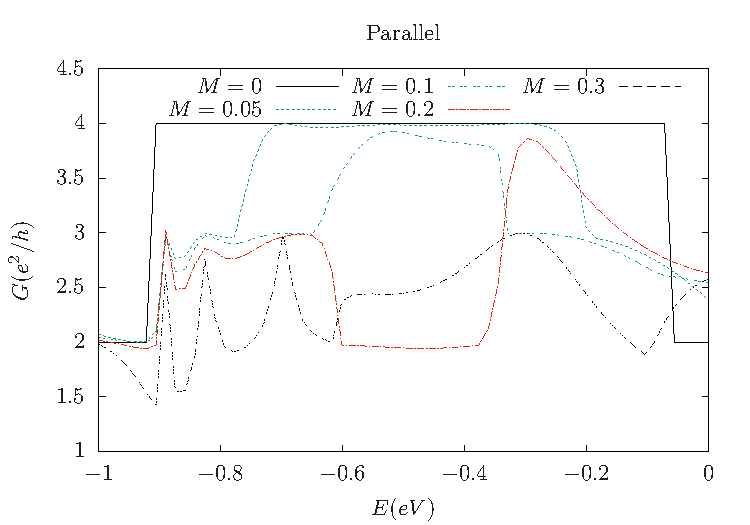
\includegraphics[width=0.45\linewidth]{../figures/armchair-parallel-conductance-1to0-revise-thesis.eps}
		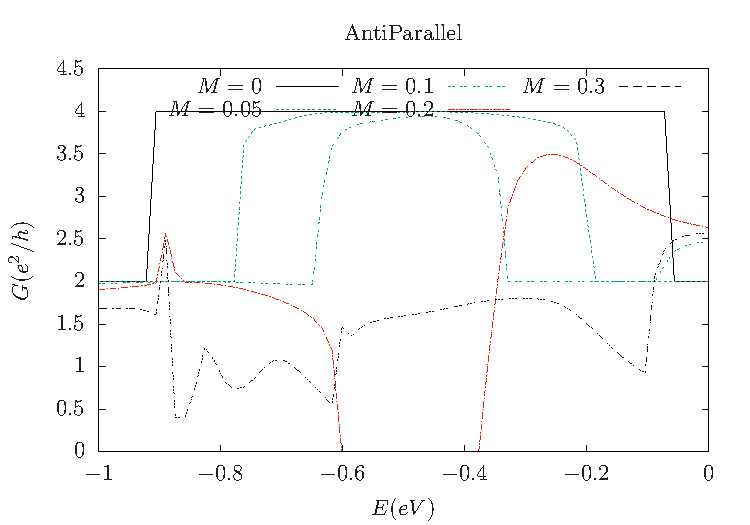
\includegraphics[width=0.45\linewidth]{../figures/armchair-antiparallel-conductance-1to0-revise-thesis.eps}
	  \end{figure}
\end{frame}
% ----------------------------------------------
% \begin{frame}{parallel-conductance}
% 	\begin{columns}[t]
% 		\begin{column}[t]{0.5\linewidth}
			
% 		\end{column}
% 		\begin{column}[t]{0.5\linewidth}
% 			\begin{figure}[ht]
% 				\raggedleft
% 				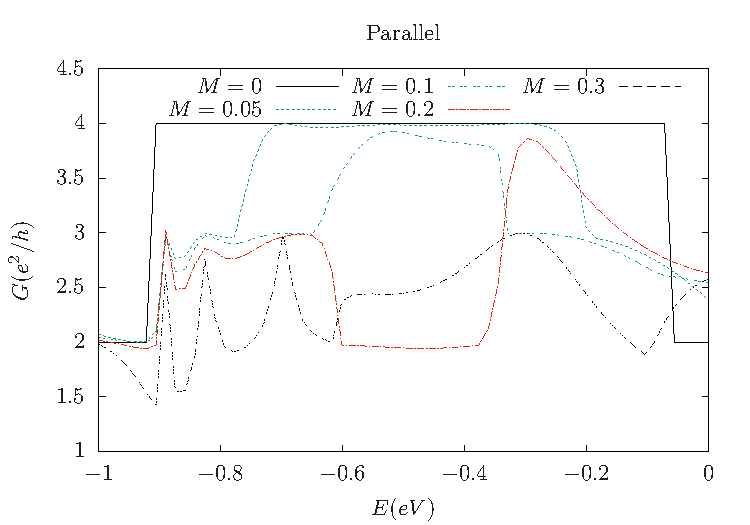
\includegraphics[width=0.9\linewidth]{../figures/armchair-parallel-conductance-1to0-revise-thesis.eps}\\
% 				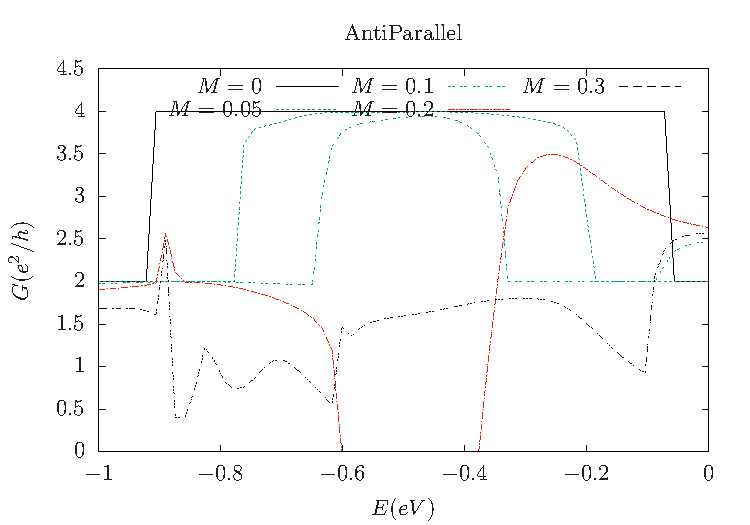
\includegraphics[width=0.9\linewidth]{../figures/armchair-antiparallel-conductance-1to0-revise-thesis.eps}
% 			  \end{figure}
% 		\end{column}
% 	\end{columns}
% \end{frame}
% -----------------------------------------------
\begin{frame}
	\begin{itemize}
		\item The difference between the P and AP configurations in zigzag borophene is much less than in armchair borophene, suggesting that zigzag borophene may be less valuable for spin valve devices.
		\item 
	\end{itemize}
\end{frame}
% end of subsection
% -----------------------------------------------
\subsection{Magnetoresistance}
% -----------------------------------------------
\begin{frame}{MR}
	\begin{itemize}
		\item Examining MR provides an important criterion for the possibility of using a device as an appropriate spin valve.
		\item When there are plateaus of 100\% in the MR diagram, the conductance in the AP configuration becomes zero, and the conductance is about one G0 in the P configuration.
		\item The description of the plateau width of the MR diagram depends entirely on the two factors that determine the conductance zeros.
	\end{itemize}
	\begin{figure}[ht]
		\centering
		\includegraphics[width=0.45\linewidth]{../figures/MR_zig-revise-thesis.eps}
		\includegraphics[width=0.45\linewidth]{../figures/MR-revise-thesis.eps}
	\end{figure}

\end{frame}
% end of subsection
% ----------------------------------------------
\subsection{Spin Transfer Torque}
% ----------------------------------------------
\begin{frame}{Spin Transfer Torque (STT) in Modified Spin Valves}
	\begin{itemize}
		\item Modified spin valves based on spin transfer torque (STT) are promising for non-volatile memory with near-zero leakage power consumption and offer opportunities to supplement or replace CMOS-based Boolean logic.
		\item Spin-polarized electrons flowing from the left to the right ferromagnetic (FM) electrode may produce a torque called spin transfer torque (STT) if the magnetization is deflected by an angle.
		\item Many parameters, such as injection, detection, and spin propagation length, must be simultaneously significant and improved to be effective for the design and fabrication of complex spintronic devices.
	\end{itemize}
\end{frame}
% -----------------------------------------------
\begin{frame}{Spin Transfer Torque (STT) in Modified Spin Valves}
	\begin{itemize}
		\item The variation of torque with the relative angle ($\theta$) between the magnetizations of the FM electrodes can be fitted with a model including the first two harmonics: $a\;\sin(\theta) + b\;\sin(2\theta) + c$.
		\item As the magnetization (M) of the FM electrodes increases, the ratio of torque to voltage ($\tau_{x}/V$) increases, confirming that $\tau_x/V$ is proportional to the polarization of the FMs.
		% \item The oscillation-like behavior is actually a sinusoidal behavior with more harmonics in borophene, as opposed to graphene and silicene, which have a purely sinusoidal behavior.
	\end{itemize}
	\begin{columns}
		\begin{column}[t]{0.5\linewidth}
			\begin{figure}[ht]
				\raggedleft
				\includegraphics[width=\linewidth]{../figures/stt-thesis.eps}
			\end{figure}
		\end{column}
		\begin{column}[t]{0.5\linewidth}
			\begin{table}[t]
				\raggedright
				\label{tbl:fitting}
				\resizebox{\textwidth}{!}{
				\begin{tabular}{lcccc}
					\toprule
					M(eV) & a & b & c \\
					\midrule
					M = 0.3 & 0.0649309- & 0.0726612 & 2.52642e-05 \\
					M = 0.2 & 0.00900465 & 0.0655489 & 3.70375e-05- \\
					M = 0.2 & 0.205575 & 0.0879828 & 0.00388147- \\
					M = 0.05 & 0.200799 & 0.0728197 & 0.00673132- \\
					\bottomrule
					\end{tabular}}
				\end{table}
		\end{column}
	\end{columns}
\end{frame}
% -----------------------------------------------
\begin{frame}{STT in Modified Spin Valves}
	\begin{itemize}
		\item The larger the difference between spin-up and spin-down transmissions, the sharper the peaks are seen.
		\item The oscillation-like behavior is actually a sinusoidal behavior with more harmonics in borophene, as opposed to graphene and silicene, which have a purely sinusoidal behavior.
		\item 
	\end{itemize}
\end{frame}
% -----------------------------------------
\begin{frame}{ُSTT VS Energy}
	\begin{itemize}
		\item The existence of energies at which the up and down spins have different energy spectra is a necessary condition for the operation of spintronic devices.
		\item The presence of more peaks in an energy range in the STT diagram indicates the energies at which the up and down spins are separated from each other.
		\item Although the order in the STT curve of graphene may not be seen in borophene, this diversity and dispersion of peaks provide more possibilities for controlling the spin separation.
	\end{itemize}
	\begin{figure}
		\centering
		\includegraphics[width=0.33\linewidth]{../figures/stt-energy3d-01-thesis.eps}
		\includegraphics[width=0.33\linewidth]{../figures/stt-energy3d-02-thesis.eps}\includegraphics[width=0.33\linewidth]{../figures/stt-energy3d-03-thesis.eps}
	\end{figure}
\end{frame}
% ---------------------------------------------

% end subsection
%-------------- Begin references
\section{References}
\begin{frame}{References}
\begin{itemize}
\item $1^{st}$ reference
\end{itemize}
\end{frame}
%------End references-----

\end{document}
